\documentclass[runningheads,12pt]{llncs}
\usepackage{graphicx}
\usepackage{float}
\usepackage{todonotes}
\usepackage{fancyhdr}
\usepackage{lipsum}
\usepackage{tabularx}
\usepackage{array}
\usepackage{longtable}
\usepackage[T1]{fontenc}
\usepackage[provide=*,english,polish]{babel}

\newcolumntype{C}[1]{>{\centering\arraybackslash}m{#1}}

\setcounter{tocdepth}{4}
\setcounter{secnumdepth}{4}
\renewcommand{\headrulewidth}{0pt}

\begin{document}

\title{Współdzielenie kodu w mikroserwisach} \subtitle{}

\author{Artem Romanenko \ Numer albumu: S32237 \inst{}}
\authorrunning{ }
\titlerunning{Your thesis title abbreviated.}
\institute{\textbf{Polish-Japanese Academy of Information Technology} \ Promotor: dr Krzysztof Barteczko, prof. PJATK}

\maketitle

\thispagestyle{fancy}

\begin{figure}[t!]
    \centering
    
\includegraphics[width=\linewidth]{images/Logo_EN_1.png}
    \label{fig:my_label}
\end{figure}

\selectlanguage{polish}
\cfoot{ Warszawa, \today}

\clearpage

\makeatletter
\renewcommand*\l@author[2]{}
\renewcommand*\l@title[2]{}
\makeatletter

\selectlanguage{english}
\begin{abstract}
Rapid development and adoption of microservices architecture in the last few years has changed the world of Informatics. Microservices architecture has many advantages, such as flexibility, fast and comfortable deployment, and easy maintenance. However, this architecture also causes new challenges, such as code duplication and complicated code management. In my master's thesis, I've carried out a deep and detailed analysis of all available approaches to manage shared code in systems of microservices. In my work, I want to compare all available approaches for sharing code in systems of microservices using literature sources and prepared code laboratory, also to define cases in which it is better to choose one or another approach. The aim is to present an approach to sharing code, combining the advantages of all existing solutions and providing better performance and convenience for developers in managing code. At the end of my work, I will place a comparison of my solution with existing solutions using prepared performance tests.
\keywords{Microservices Architecture \and Code Sharing \and Performance.}
\end{abstract}

\newpage

\selectlanguage{polish}
\begin{abstract}
Z pewnością szybki rozwój i przyjęcie architektury mikroserwisowej w ostatnich latach zmieniły świat informatyki. Uważam, że architektura mikroserwisowa ma wiele zalet, takich jak na przykład elastyczność, prostota wdrożenia i utrzymania. Jednak powoduje nowe wyzwania dla programistów, takie jak na przykład problem duplikacji kodu. W pracy magisterskiej przeprowadziłem dokładną analizę metod i podejść współdzielenia kodu w systemach mikroserwisów, porównałem za pomocą źródeł literaturowych oraz przeprowadzonych badań dostępne podejścia do współdzielenia kodu, zdefiniowałem przypadki, w których należy wybrać określone podejście. W części praktycznej zaprezentowałem własne nowoczesne rozwiązanie, które łączy zalety istniejących rozwiązań, wydajność oraz komfort zarządzania kodem. Na końcu umieściłem porównanie mojego rozwiązania z istniejącymi za pomocą przygotowanych testów wydajnościowych.
\keywords{Architektura mikrousług \and Współdzielenie kodu \and Wydajność.}
\end{abstract}

\newpage

\tableofcontents

\newpage

\section{Wstęp}

\subsection{Zakres pracy}
W pracy magisterskiej przeprowadzono dokładną analizę metod i podejść do współdzielenia kodu w systemach mikroserwisów. Zakres tej pracy zawiera porównanie między architekturą monolitową a mikroserwisową, identyfikację typów obiektów wykorzystywanych w kodzie współczesnych aplikacji, analizę dostępnych metod i podejść do współdzielenia kodu, IDL, SDK oraz biblioteki, a także praktyczną implementację aplikacji wspierającej nowatorskie podejście do współdzielenia kodu Serverless.

\subsection{Motywacja}
Główną motywacją do napisania pracy było rosnące we współczesnych czasach zainteresowanie mikroserwisowym podejściem do architektury, które ma wiele zalet, takich jak elastyczność, łatwość wdrożenia i utrzymania na produkcji, możliwość łatwej i szybkiej naprawy problemów na produkcji, natomiast również powoduje nowe wyzwania, takie jak problem duplikacji kodu i zapotrzebowanie na współdzielenie kodu między mikroserwisami w systemie.
W mojej pracy chcę przeanalizować, jakie metody współdzielenia kodu są dostępne na rynku, jakie są ich zalety i wady, jakie są najlepsze praktyki we współdzieleniu kodu w systemach mikroserwisów. Chcę porównać bardziej tradycyjne podejścia do współdzielenia kodu, takie jak IDL, SDK, biblioteki, z nowatorskim podejściem do współdzielenia kodu, takim jak Serverless, chcę stworzyć oprogramowanie, które połączy główne zalety tradycyjnych metod współdzielenia kodu z zaletami bardziej nowoczesnych podejść.

\newpage

\subsection{Zawartość pracy}
Praca jest ustrukturyzowana w kilka rozdziałów, przedstawiam krótki opis rozdziałów pracy:
\begin{enumerate}
    \item Wstęp - W tym rozdziale analizuję wady i zalety architektury mikroserwisowej oraz monolitycznej, też analizuję, dlaczego z architektury monolitycznej powstała w ostatnich latach architektura mikroserwisowa, przeprowadzam analizę przypadków, w których lepiej użyć architektury monolitycznej a w których architekturę mikroserwisową. Opisuję, dlaczego powstało zapotrzebowanie na współdzielenie kodu. Uzasadniam informację przykładami z literatury.
    \item Architektura mikroserwisowa a Monolityczna - W tym rozdziale pracy porównam mikroserwisy z podejściem monolitycznym, przedstawiam różnice w utrzymaniu i skalowalności, za pomocą źródeł literaturowych.
    \item Analiza dziedziny problemowej - W tym rozdziale przedstawiam kategoryzuję typy obiektów które mogą potrzebować współdzielenia kodu w systemie mikroserwisów, analizuję możliwe wyzwania związane z współdzieleniem poszczególnych typów obiektów, przedstawiam uzasadnienia z literatury.
    \item Analiza metod współdzielenia kodu - W tym rozdziale kompleksowa analiza istniejących metod współdzielenia kodu w systemach mikroserwisów za pomocą kryteriów oceny opartych na źródłach literaturowych.
    \item Opis części praktycznej - Zawiera opis przygotowanej w ramach pracy aplikacji, która wspomaga nowoczesne rozwiązanie do współdzielenia kodu w systemach mikroserwisów - Serverless rozszerzając możliwości tego rozwiązania.
\end{enumerate}

\newpage

\section{Ogólna definicja współdzielenia kodu}

Współdzielenie kodu – to praktyka w programowaniu polegająca na udostępnianiu fragmentów kodu lub całych funkcji, metod albo modułów – w zależności od architektury i użytych technologii – między różnymi projektami, zespołami, a czasem również między firmami lub społecznościami open source.

Celem współdzielenia kodu jest:

\begin{enumerate}
    \item Unikanie duplikacji – możliwość wielokrotnego użycia fragmentu kodu w różnych miejscach.
    \item Zwiększenie produktywności – możliwość szybkiego korzystania z gotowych rozwiązań.
    \item Utrzymanie spójności – pozwala na stosowanie jednolitych reguł wewnątrz aplikacji oraz między aplikacjami, takich jak na przykład reguły walidacji, formatowania danych czy też obsługi błędów.
    \item Ułatwienie współpracy zespołowej – ułatwia korzystanie z wyników pracy jednego programisty przez zespół oraz między zespołami.
    \item Lepsze testowanie i jakość – ze względu na utrzymanie spójnych reguł w aplikacji kod jest łatwiejszy do testowania, co zmniejsza ryzyko błędów i poprawia ogólną jakość kodu.
\end{enumerate}

W przypadku architektury mikroserwisowej współdzielenie kodu to praktyka udostępniania fragmentów kodu – na przykład bibliotek, modułów, metod lub funkcji – pomiędzy mikroserwisami (elementami systemu mikroserwisowego), w celu osiągnięcia korzyści przedstawionych powyżej. W przypadku architektury monolitycznej współdzielenie kodu również odgrywa ważną rolę w utrzymaniu jakości kodu i aplikacji.

\section{Architektura mikroserwisowa a monolityczna}

Mikroserwisowa infrastruktura, szybko rozwijająca się w ostatnich latach, przyniosła wiele korzyści w świat informatyki. Pozwoliła na tworzenie skalowalnych i elastycznych systemów, ułatwiła utrzymanie takich systemów. Natomiast musimy również uważać przy wyborze architektury na to, że w przypadku mikroserwisów musimy poradzić sobie z kwestią współdzielenia kodu w takim systemie mikroserwisów.

\subsection{Architektura mikroserwisowa}

Na podstawie mojego doświadczenia, podział aplikacji na mniejsze, niezależne usługi przynosi liczne korzyści. Każdy mikroserwis można skalować osobno, co pozwala na poprawę wydajności całego systemu. W sytuacji, gdy pojawia się problem, naprawa jest prostsza, ponieważ wystarczy skupić się na jednej części aplikacji, a nie na całym systemie. Mikrousługi wpływają również na organizację pracy zespołowej. Deweloperzy mogą skupić się na rozwoju pojedynczych mikroserwisów, co ułatwia zarządzanie projektem i zmniejsza ryzyko wystąpienia błędów w innych częściach aplikacji. Ponadto, gdy pojawia się problem, jest on łatwiejszy do zidentyfikowania, a proces naprawy staje się bardziej efektywny. Kolejną zaletą mikrousług, moim zdaniem, jest ich elastyczność pod względem doboru technologii. Dzięki temu, że każdą usługę można tworzyć i zarządzać nią z użyciem różnych narzędzi, istnieje większa swoboda w doborze najlepszych rozwiązań technologicznych do każdej części systemu. Mikrousługi wspierają również skuteczne zarządzanie projektem, ponieważ umożliwiają szybsze wdrażanie nowych funkcji i reagowanie na zmiany. Taki system jest bardziej odporny na awarie, a cały proces utrzymania aplikacji jest prostszy. ~\cite[p. 2]{newman2015building}

Architektura mikrousług przedstawia następujące cechy:

\begin{enumerate}
    \item Modułowość - W przypadku mikroserwisów możemy wdrażać pojedyncze elementy systemu bez wpływu na pozostałe.
    \item Niezawodność - Mikroserwisy są niezawodne, ponieważ błąd w jednej części systemu niekoniecznie będzie miał wpływ na cały system.
    \item Interoperacyjność — Komunikacja za pomocą wymiany danych przez zasoby sieciowe daje nam możliwość połączenia mikroserwisów napisanych w różnych językach i technologiach. W tym przypadku możemy połączyć w jednym systemie kilka technologii i wykorzystać mocne strony każdej z nich.
    \item Równoległy rozwój - Zespoły programistów mogą pracować nad osobnymi mikroserwisami równolegle, bez konfliktów zmian w kodzie.
\end{enumerate}

\subsection{Architektura monolityczna}

Charakterystyka architektury monolitycznej:

\begin{enumerate}
    \item Wdrożenie - Cała aplikacja jest wdrażana jako całość, niepodzielna jednostka. Wszystkie aktualizacje wymagają wdrożenia całej aplikacji.
    \item Kontrola przepływu kodu - Centralny moduł kontroli w aplikacji koordynuje sekwencyjne wykonywanie kodu.
    \item Powiązanie - Poszczególne elementy aplikacji są ściśle powiązane.
    \item Współdzielona pamięć - Wszystkie komponenty oprogramowania mają bezpośredni dostęp do zasobów, co sprzyja ich integracji, natomiast taka konfiguracja może powodować konflikty elementów kodu na poziomie sprzętowym i trudności ze skalowaniem. \cite{sharma2023monolithic}
\end{enumerate}

\subsection{Porównanie}

Zalety architektury monolitycznej:

\begin{itemize}
    \item Czas napisania – Dla małych i średnich projektów umożliwia szybsze napisanie kodu bez potrzeby zarządzania komunikacją między mikroserwisami w systemie.
    \item Łatwość wdrożenia – Wdrożenia kodu w przypadku architektury monolitycznej są mniej skomplikowane.
    \item Proste testowanie – O wiele łatwiejsze jest testowanie aplikacji monolitycznej dzięki ścisłej integracji wszystkich komponentów. Testy jednostkowe i integracyjne można w prosty sposób przeprowadzać w ramach pojedynczej bazy kodu.
    \item Skalowalność – Zapewnia odpowiednią skalowalność dla niewielkich rozwiązań poprzez replikację całej aplikacji.
\end{itemize}

Zalety architektury mikroserwisowej:

\begin{enumerate}
    \item Skalowalność - Mikroserwisy umożliwiają niezależne skalowanie, optymalizując wykorzystanie zasobów i zapewniając wydajność systemu.
    \item Równoległa praca - Architektura mikroserwisowa pozwala na równoległy rozwój kilku elementów systemu bez konfliktów, co prowadzi do szybszego rozwoju.
    \item Elastyczność - Każdy mikroserwis może być napisany w języku najbardziej pasującym do jego konkretnej funkcji, daje to możliwość użycia mocnych stron każdej z wielu dostępnych technologii.
    \item Debugowanie - Rozwiązywanie problemów w mikroserwisach jest prostsze, każdy osobny mikroserwis jest niewielki i prosty w analizie.
    \item Bezpieczeństwo - Mikroserwisy ułatwiają ochronę danych. Każda usługa ma swoją bazę danych, co utrudnia hakerom dostanie się do danych.~\cite{sharma2023monolithic}
\end{enumerate}

Wybór między architekturą monolityczną a mikroserwisową zależy od wielu faktorów, takich jak rozmiar projektu, zapotrzebowanie na ciągły rozwój, wymagania dotyczące skalowalności oraz kompetencje i doświadczenia zespołu. Architektura monolityczna lepiej pasuje dla małych i mniej skomplikowanych projektów natomiast mikroserwisowa oferuje benefity w przypadku wykorzystania w większych, bardziej skomplikowanych systemach. ~\cite[p. 11]{newman2015building}

\newpage

\section{Analiza dziedziny problemowej}

Celem niniejszej pracy magisterskiej jest zgłębienie tematu współdzielenia obiektów w systemach mikroserwisów oraz zrozumienie wyzwań i możliwości związanych z tym zagadnieniem. Praca ma na celu analizę różnych strategii, narzędzi i metodyk, które mogą pomóc w efektywnym i bezpiecznym współdzieleniu danych i obiektów w skali mikroserwisowej architektury.

\subsection{Typy obiektów w aplikacjach mikroserwisowych}

Postanowiłem rozpocząć analizę dziedziny problemowej od tego, że za pomocą źródeł literaturowych zidentyfikuję typy obiektów oraz dokonam analizy tego, które z nich mogą wymagać współdzielenia w systemach mikroserwisów.

\begin{enumerate}
    \item DTO (Data Transfer Object) - Takie obiekty są specjalnie przeznaczone do obsługi przesyłania danych między elementami systemu mikroserwisów, są lekkie i nie zawierają logiki biznesowej, dlatego współdzielenie takich obiektów jest jak najbardziej zalecane, ponieważ zapewniają spójność danych po obu stronach komunikacji oraz zmniejszają ilość błędów w przypadku rozwoju lub utrzymania aplikacji.
    \item Model (lub Encja) - Najczęściej są logicznie powiązane z tabelami w bazie danych, ze względu na to, że we współczesnych czasach za dobrą praktykę jest uważane podejście, w którym jeden mikroserwis jest powiązany z maksymalnie jedną bazą danych, współdzielenie tego typu obiektów nie jest zalecane.
    \item Wyjątek (Exception) - Zalecanym jest współdzielenie informacji o wyjątkach w systemie mikroserwisów, tym samym tworząc jednolitą obsługę błędów w systemie. Logika związana z obsługą błędów, w przypadku podobności w kilku serwisach też jest dobrym kandydatem do współdzielenia. Taka standaryzacja w systemie mikroserwisów sprawia, że łatwiej później znaleźć źródło błędu i naprawić go.
    \item Walidatory - W przypadku współdzielenia walidatorów w systemie mikroserwisów można zapewnić integralność danych w całym systemie oraz zmniejszyć duplikację kodu, również standaryzacja walidacji obiektów w systemie zmniejsza ilość ewentualnych problemów w trakcie ewolucji i rozwoju mikroserwisów w przyszłości. Współdzielenie takich obiektów jest dobrą praktyką i jest zalecane.
    \item Serwisy - W przypadku logiki, która powtarza się w dwóch i więcej serwisach, zalecanym jest współdzielenie takiego serwisu za pomocą najlepiej w tym przypadku pasującej metody. Zmniejsza to duplikację kodu, natomiast zwiększa czytelność i spójność kodu w systemie mikroserwisów, zmniejsza ilość ewentualnych problemów w trakcie ewolucji i rozwoju kodu.
\end{enumerate}

Musimy zdawać sobie sprawę, że mimo tego, iż współdzielenie kodu daje nam wiele korzyści, nadmiarowe współdzielenie kodu może spowodować problemy i pogorszyć jakość oraz zrozumiałość naszego kodu, utrudnić testowanie, spowodować powstanie błędów kaskadowych, czyli sytuacji, kiedy błąd w jednym źródle powoduje problemy od razu w wielu miejscach, oraz utrudnić utrzymanie systemu. Należy zawsze używać współdzielenia ostrożnie i podejmować decyzję w każdym konkretnym przypadku współdzielenia.

\newpage

\subsection{Kryteria porównania i analizy metod współdzielenia kodu}

Po przeprowadzeniu dogłębnej analizy tematu i między innymi źródeł literaturowych, takich jak ~\cite{newman2015building}, ~\cite{richardson2018microservices}, ~\cite{nygard2008release}, ~\cite{kleppmann2017designing} mogę zdefiniować kryteria porównania metod współdzielenia kodu w systemach mikroserwisów jako następujące:
% AI
\begin{enumerate}
    \item Komunikacja - Metoda współdzielenia obiektów powinna uwzględniać efektywną komunikację między serwisami. Ważne jest, aby obiekty były dostępne w sposób, który minimalizuje opóźnienia i obciążenie sieci. Dobre rozwiązania mogą obejmować użycie asynchronicznej komunikacji, takiej jak kolejki wiadomości, czy też bezpośrednie zapytania między serwisami.
    \item Izolacja - Metoda współdzielenia obiektów powinna zapewniać odpowiednią izolację między serwisami. Każdy serwis powinien mieć kontrolę nad swoimi własnymi obiektami i nie powinien być zależny od innych serwisów. To pozwala na większą elastyczność i umożliwia niezależny rozwój i skalowanie serwisów.
    \item Bezpieczeństwo - W przypadku współdzielenia obiektów, istotne jest zapewnienie odpowiedniego poziomu bezpieczeństwa. Dostęp do obiektów powinien być kontrolowany i zabezpieczony w sposób, który zapobiega nieautoryzowanemu dostępowi. Mechanizmy uwierzytelniania i autoryzacji powinny być odpowiednio wdrożone, aby zapewnić bezpieczne współdzielenie obiektów.
    \item Skalowalność - Metoda współdzielenia obiektów powinna być skalowalna. System powinien być w stanie efektywnie obsługiwać rosnącą liczbę żądań i zapewniać odpowiednią wydajność. Współdzielenie obiektów powinno być projektowane w taki sposób, aby możliwe było łatwe skalowanie poszczególnych serwisów bez wpływu na cały system.
    \item Wersjonowanie - Ważne jest również odpowiednie zarządzanie wersjami obiektów, szczególnie w środowisku mikroserwisów, gdzie różne serwisy mogą używać różnych wersji obiektów. Metoda współdzielenia obiektów powinna uwzględniać zarządzanie wersjami i umożliwiać aktualizacje w sposób kontrolowany i bezpieczny.
\end{enumerate}

\newpage

\section{Analiza metod współdzielenia kodu}

We współczesnych czasach współdzielenie kodu jest niezbędne w skomplikowanych systemach mikroserwisów, w tym rozdziale pracy porównuję istniejące podejścia do współdzielenia kodu oraz porównuję je za pomocą zdefiniowanych w poprzednim rozdziale kryteriów. Głównym celem jest zdefiniowanie najlepszych praktyk współdzielenia kodu, określenie, które podejście jest najbardziej dopasowane do współdzielenia konkretnych typów obiektów, zdefiniowanych powyżej w tej pracy oraz porównanie wydajności i możliwości skalowania w przypadku każdego z podejść za pomocą przygotowanych programistycznych testów wydajnościowych.

\subsection{Metody współdzielenia kodu z opisem}

Za pomocą źródeł literatury oraz własnego doświadczenia zdefiniowałem dostępne na dzień dzisiejszy podejścia:

\begin{enumerate}
    \item Interface definition languages - do IDL należy wiele popularnych technologii, Protocol buffers, Avro IDL, Open API. ~\cite{wiki:interface_description_language}
    \item Biblioteki kodu - najbardziej oczywiste podejście, które daje możliwość współdzielenia wszystkich rodzajów obiektów w aplikacji.
    \item Biblioteki klienckie - podejście które polega na udostępnieniu za pomocą biblioteki kodu zestawu obiektów potrzebnych do komunikacji z narzędziem zewnętrznym, takim jak, na przykład konsola AWS.
    \item Wyniesienie kodu do osobnego REST serwisu - podejście polega na przechwytywaniu i udostępnieniu wspólnej logiki poprzez utworzenie osobnego mikroserwisu.
    \item Serverless - nowoczesne podejście do pisania kodu i przetwarzania informacji wykorzystywane w chmurach obliczeniowych. Pozwala na uruchamianie kawałków kodu, metod i funkcji niezależnie, bez warstwy zarządzania aplikacją, a także na uruchamianie kodu bez konieczności zarządzania podstawową infrastrukturą. ~\cite{ibm_serverless}
\end{enumerate}
% AI
Pryncypia działania poszczególnych metod współdzielenia kodu:

Interface definition languages – są powszechnie używane w oprogramowaniu zdalnych wywołań procedur. W takich przypadkach maszyny po obu stronach łącza mogą używać różnych systemów operacyjnych i języków programowania. IDL oferują most pomiędzy dwoma różnymi systemami. Natomiast również mogą być użyte dla generacji obiektów lub kodów w systemach mikroserwisów. Każdy system IDL posiada określony przez twórców język IDL oraz interpretator języka IDL. Interpretator języka IDL przygotowany i dostarczony przez twórców potrafi na podstawie udostępnionych reguł wygenerować kod używając przygotowane pliki IDL. Używając języka IDL możemy przygotować obiekty lub kod zapisany za pomocą języka IDL, a później udostępnić przygotowane pliki IDL nieograniczonej ilości mikroserwisów i na podstawie udostępnionych plików wygenerować w każdym z mikroserwisów kod lub obiekty, które zostaną użyte przez specyficzną logikę konkretnego serwisu dla osiągnięcia konkretnego celu biznesowego. Tworzenie kodu na podstawie plików IDL jest łatwo zautomatyzowane za pomocą narzędzi do budowania aplikacji, takich jak Gradle czy Maven, dlatego możemy używać IDL jako metodę współdzielenia kodu. W trakcie pracy zamierzam sprawdzić skuteczność tej metody, problemy związane z jej użyciem oraz określić przypadki, w których dobrze się nadaje, jak również przypadki, w których lepiej jej nie stosować.

Libraries – biblioteki to w odpowiedni sposób przygotowany kod, który my za pomocą odpowiednich narzędzi możemy łatwo importować i używać jako część innego programu. Program importujący bibliotekę może używać kodu biblioteki tak, jakby to był własny kod programu. Istnieje wiele narzędzi, które wspomagają łatwe i szybkie importowanie i zarządzanie bibliotekami kodu, takie jak Maven czy Gradle. W współczesnych systemach mikroserwisów współdzielenie kodu za pomocą bibliotek kodu odbywa się za pomocą serwisów do przechowywania artefaktów i plików binarnych, takich jak Nexus. ~\cite[5]{labouardy2021pipeline} Na pierwszym etapie narzędzie do budowania projektu przygotowuje bibliotekę i wysyła ją na serwer. Dalej kod może być przechowywany nieograniczoną ilość czasu na serwerze. Aplikacje, które mają dostęp do serwera, mogą pobrać bibliotekę z kodem i przechowywać w lokalnym systemie plików, używając jako część kodu źródłowego. Biblioteka może być udostępniona nieograniczonej liczbie projektów. Organizacja może ograniczać dostęp do serwera.

SDK – mechanizm działania podobny do bibliotek, różni się jedynie podejściem. W przypadku kodu SDK na serwerze udostępniającym dependencje przechowywane są jedynie obiekty, które muszą być użyte do komunikacji z innym programem lub kodem. Logika biznesowa nie została udostępniona w takim przypadku i zostaje ukryta oraz nie może zostać zmieniona. W przypadku udostępnienia SDK możemy łatwo zapewnić bezpieczeństwo kodu (użytkownicy wciągający dependencje nie widzą logiki biznesowej) oraz chronimy się przed przypadkowymi oraz niepożądanymi zmianami kodu. Pozwala to zaoszczędzić na testach manualnych oraz automatycznych kodu. Przykład, w którym możemy użyć współdzielenia kodu SDK to – mamy mikroserwis, który udostępnia API. API przyjmuje obiekty JSON, które mogą być opisane za pomocą obiektów Java. Obiekty, które pozostałe mikroserwisy w systemie mikroserwisów mogą użyć do wysłania żądań do określonego wcześniej mikroserwisu udostępniającego API, możemy udostępnić dla naszego systemu mikroserwisów jako bibliotekę. Każdy serwis, który chce wysyłać żądania do serwisu REST-owego, może pobrać bibliotekę w postaci dependencji za pomocą narzędzia do budowania i użyć przygotowane obiekty do komunikacji. Natomiast kod serwisu nie zostanie udostępniony. W ramach prac nad serwisem korzystającym z API REST-owego nie musimy testować kodu API, bo on nie został udostępniony i dlatego nie mógł ulec zmianie w trakcie pisania kodu serwisu.

REST API - Representational State Transfer Application Programming Interface jeden z najpopularniejszych podejść do komunikacji między mikroserwisami i dla współdzielenia kodu w systemach mikroserwisów. Przykładami współdzielenia kodu za pomocą REST mogą być mikroserwis do uwierzytelniania użytkowników, który może być wykorzystany przez każdy serwis w systemie mikroserwisów, tym samym logika związana z uwierzytelnieniem użytkowników jest współdzielona między elementami systemu. REST API pozwala na kompletne odseparowanie współdzielonego kawałka logiki od implementacji aplikacji, tym samym redukując problemy związane z zarządzaniem wersjami, które występują w przypadku bibliotek i SDK. Również współdzielenie kodu za pomocą REST API nie powoduje zależności i sztywnych powiązań między mikroserwisami, co sprawia, że system jest bardziej elastyczny, natomiast trudniej w takim przypadku utrzymać spójność API kontraktów w systemie. Współdzielenie kodu za pośrednictwem interfejsu API REST obejmuje udostępnianie danych lub funkcji za pomocą standardowych metod HTTP (GET, POST, PUT, DELETE) i wymianę informacji w formatach takich jak JSON lub XML. Do zalet podejścia można odnieść dobrą skalowalność, nowe mikroserwisy mogą być łatwo dodawane i usuwane bez wpływu na cały system, również REST API pozwala na lepszy i bardziej zrozumiały podział odpowiedzialności w systemie, co prowadzi do zmniejszenia duplikacji kodu. Do wad tego podejścia możemy odnieść trudności w utrzymaniu, w przeciwieństwie do bibliotek i SDK zmiany w API nie są automatycznie wykrywane przez klientów, również różni klienci mogą równocześnie używać różnych wersji API, co wymaga mechanizmów kontroli wersji.

Serverless - Nowoczesne podejście, które pozwala na uruchamianie kodu bez bezpośredniego zarządzania infrastrukturą i sprzętem. W przypadku tego podejścia chmura obliczeniowa zarządza przydzieleniem odpowiednich zasobów, zarządza skalowaniem i utrzymaniem serwera, dając możliwość programiście skupić się na napisaniu kodu. W kontekście współdzielenia kodu, serverless pozwala na stworzenie małych, niezależnych funkcji, które mogą być łatwo wykorzystane do współdzielenia kodu w systemach mikroserwisów. Takie podejście dobrze pasuje do współdzielenia małych, często powtarzających się kawałków kodu. Technologia serverless również pozwala usprawnić współpracę między zespołami, zmniejsza duplikację kodu i upraszcza konserwację. Funkcje współdzielone za pomocą serverless mogą być udostępniane za pomocą technologii REST, co wiąże się z wszystkimi zaletami i wadami tego podejścia, albo za pomocą SDK udostępnionego przez dostawcę chmury.

\subsection{Analiza metod współdzielenia kodu dla różnych typów obiektów}

Po przeprowadzeniu analizy źródeł literaturowych oraz własnego doświadczenia dokonałem analizy tego, jakie metody współdzielenia mogą zostać wykorzystane dla poszczególnych typów obiektów.

Obiekty DTO (Interface Definition Languages) mogą być współdzielone za pomocą IDL, generowanie obiektów na podstawie plików IDL pozwala na standaryzację kontraktów komunikacji między mikroserwisami. Również obiekty DTO mogą być współdzielone za pomocą bibliotek, takie obiekty mogą albo bezpośrednio w bibliotekach, albo pliki IDL, na podstawie których później będą wygenerowane klasy DTO, mogą być udostępniane za pomocą bibliotek. Takie podejście jest często wykorzystywane w procesach CI/CD. SDK też jest dobrze dopasowanym podejściem wykorzystywanym razem z obiektami DTO, udostępnienie obiektów DTO za pomocą SDK bez udostępniania bezpośrednio logiki biznesowej jest dobrą praktyką w programowaniu. Współdzielenie obiektów DTO może zapewnić to, że zakłada usługa będzie wykorzystywać spójne struktury danych, ułatwiając komunikację, zmniejszając tym samym ryzyko niespójności.

Obiekty Model, współdzielenie takich obiektów zgodnie z wcześniejszą analizą nie jest zalecane, ze względu na to, że zalecane jest wykorzystywanie nie więcej niż jednej bazy dla każdego mikroserwisu. Ze względu na to, nie można znaleźć najlepszej opcji do współdzielenia takich obiektów. Teoretycznie obiekty Model mogą być współdzielone za pomocą bibliotek, ale jak zaprezentowano w ~\cite{bhuyan2020microservices}, może to powodować później problemy z zarządzaniem kodem i środowiskami.

Walidatory, jako obiekty zawierające w ograniczonej skali logikę programu, mogą być współdzielone za pomocą bibliotek, REST API oraz technologii Serverless. Współdzielenie walidatorów jest dobrą praktyką i jest zalecane, ponieważ pozwala na utrzymanie spójnych reguł walidacji w systemie mikroserwisów, co poprawia jakość danych, które wymieniają się elementy systemu. W przypadku współdzielenia za pomocą bibliotek, tracimy możliwość połączenia kilku mikroserwisów napisanych w różnych językach programowania w jeden system mikroserwisów, co natomiast możemy zrobić w przypadku współdzielenia za pomocą REST oraz Serverless. Serverless jest najlepszą opcją współdzielenia walidatorów, ze względu na to, że walidatory zawierają zwykle niewielką ilość logiki, która mieści się w jednej funkcji, którą idealnie nadają się do hostowania za pomocą Serverless. Również w tym przypadku nie tracimy możliwości połączenia kilku mikroserwisów napisanych w różnych językach programowania w jeden system mikroserwisów.

Serwisy, serwisami są głównym miejscem przechowywania, serwisy mogą być współdzielone za pomocą bibliotek, SDK, REST oraz Serverless. W przypadku wyboru podejścia do współdzielenia mikroserwisów należy dokonać analizy i zastanowić się. Biblioteki kodu są najbardziej uniwersalnym podejściem w przypadku serwisów, pasują do wykorzystania w przypadku współdzielenia małych metod zawierających małą ilość kodu, jak i tych większych. Podejście REST też dobrze pasuje do wszystkich form współdzielonej logiki, ale natomiast w wysoko obciążonych systemach może powodować obniżenie wydajności ze względu na rozproszenie zasobów na komunikację sieciową. Podejście Serverless dobrze się sprawdza w przypadku współdzielenia mniejszych metod, zarządzanie skomplikowaną logiką za pomocą Serverless może być skomplikowane, jak w przypadku REST, w wysoko obciążonych systemach podejście raczej trzeba zmienić na bibliotekę lub SDK.

\subsection{Definicja kryterium oceny i porównania metod współdzielenia kodu}

Na podstawie źródeł literaturowych, własnego doświadczenia oraz przygotowanych testów wydajnościowych dokonałem analizy przedstawionych powyżej podejść do współdzielenia kodu w systemach mikroserwisów.

\subsubsection{Definicja kryterium oceny pod kątem izolacji w przypadku IDL}

Przedstawiam kryteria, które wybrałem w rezultacie analizy źródeł internetowych oraz książek takich jak ~\cite{kleppmann2017designing}, w których znalazłem opis tego, jak musi wyglądać architektura mikroserwisowa, wady i zalety różnych rozwiązań.

\begin{enumerate}
    \item Conflict Rate - wskaźnik tego, jak często zmiany w plikach IDL powodują konflikty scalania (merge conflicts). Wyzwania dotyczące pracy z IDL i podejścia do ich pokonania są dobrze opisane w książce ~\cite{kleppmann2017designing}. Szczegółowo opisane są metody pracy ze schematami IDL, między innymi narzędziem Protocol Buffer rozwijanym przez Alphabet oraz Avro. To oznacza, że stare i nowe wersje kodu oraz stare i nowe formaty danych mogą potencjalnie współistnieć w systemie w tym samym czasie. Aby system działał płynnie, musimy zachować kompatybilność w obu kierunkach: kompatybilność wsteczną i kompatybilność w przód.
    Musimy uważać na to, jaką liczbę konfliktów generuje stosowanie wybranego podejścia. Takie konflikty często są czasochłonne i nawet w przypadku prostych sytuacji potrafią spowolnić zespół deweloperski oraz spowodować inne, bardziej skomplikowane błędy. ~\cite[p. 112]{kleppmann2017designing}
    \item Version Drift Occurrence - wskaźnik tego, jak często rozwiązanie powoduje użycie niezgodnych wersji IDL w różnych zespołach. Kiedy zespoły programistów pracujące nad jednym systemem zaczynają używać niezgodnych wersji plików IDL, mikroserwisy w systemie mikroserwisów przestają komunikować się poprawnie, co powoduje błędy w runtime, które są bardzo trudne do wyłapania i naprawy, nieoczekiwane zachowanie systemu oraz uszkodzenie danych. W przypadku wykorzystania podejścia, które nie może zapewnić odpowiedniego poziomu kontroli nad wersjami i izolacji, rozwój i wdrażanie zmian w systemie mogą być problematyczne.
    W przypadku braku kompatybilności nie jest możliwe poprawne działanie systemu. ~\cite[p. 123]{kleppmann2017designing}
    \item Build Failure Rate - wskaźnik tego, jak często zmiany w plikach IDL powodują problemy w trakcie budowania aplikacji.
    Problemy te często wynikają z nieprawidłowo wybranego podejścia do zarządzania plikami IDL. ~\cite[p. 123]{kleppmann2017designing}
    \item Deployment Rollback Frequency - wskaźnik tego, jak często zmiany w plikach IDL powodują problemy w trakcie wdrożenia aplikacji na środowiska w systemie mikroserwisów.
    Częste wycofywania zmian (rollbacki) usług w trakcie wdrożeń mogą spowodować spowolnienie wdrożenia nowych funkcjonalności i opóźnienie projektu, dlatego w trakcie wyboru podejścia do zarządzania plikami IDL musimy brać to pod uwagę. Musimy w trakcie analizy i planowania projektu wybrać podejście, które zapewni najmniejsze ryzyko błędów w trakcie próbnego wdrożenia i wycofania zmian. ~\cite[p. 92]{kleppmann2017designing}
\end{enumerate}

\subsubsection{Definicja kryterium oceny pod kątem izolacji w przypadku bibliotek, SDK, REST, serverless}

W kontekście bibliotek, SDK, REST i serverless znaczenie pojęcia izolacji różni się od izolacji w kontekście IDL. W tym przypadku izolacja to zdolność systemu do odseparowania komponentów systemu i zminimalizowania wpływu zmian w jednym serwisie na pozostałe, co daje podejściu mikroserwisowemu jego wygodność i elastyczność.

W przypadku izolacji na podstawie analizy źródeł literaturowych oraz własnego doświadczenia zdefiniowałem kryteria porównania jako następujące:

% AI
\begin{enumerate}
    \item Izolacja interfejsów - elementy w systemie mikroserwisów muszą zapewnić jasno określone interfejsy, które pozwolą na łatwą komunikację. Zmiany w jednym elemencie systemu nie powinny wpływać na pozostałe.
    Za pomocą tego cytatu możemy wyjaśnić, w jaki sposób dobrze zaprojektowane interfejsy umożliwiają zmiany bez wpływu na inne części systemu. ~\cite[p. 75]{bloch2018effective}
    \item Izolacja wersji - w przypadku aktualizacji, nowa wersja powinna być kompatybilna wstecznie z poprzednimi wersjami kodu. Izolacja wersji zapewnia, że stare wersje, dostarczone przez biblioteki, SDK, REST czy serverless, mogą współistnieć z nowszymi wersjami, umożliwiając stopniową aktualizację systemu.
    Powyższy cytat pokazuje, jak ważnym jest zachowanie kompatybilności wstecznej w przypadku współdzielenia kodu w systemach mikroserwisów. ~\cite[p. 172]{fowler2012patterns}
    \item Izolacja zależności - w przypadku SDK, bibliotek, REST czy serverless powinniśmy minimalizować wpływ zewnętrznych zależności na naszą aplikację.
    Powyższy cytat pokazuje, jak ważnym jest odseparowanie i izolacja zależności dla zachowania elastyczności. ~\cite[p. 218]{martin2008clean}
\end{enumerate}

\subsubsection{Definicja kryterium oceny pod kątem bezpieczeństwa}

% AI
\begin{enumerate}
    \item Poufność (Confidentiality) - Zapewnienie tego, że poufne dane nie będą udostępnione osobom lub systemom nieupoważnionym. Zachowanie poufności jest kluczowe dla ochrony danych osobowych i korporacyjnych. ~\cite[p. 22]{stallings2017cryptography}
    \item Integralność danych (Integrity) - Integralność danych koncentruje się na dokładności i wiarygodności informacji, chroniąc przed nieautoryzowanymi modyfikacjami, zapewniając, że dane są zarówno niezawodne, jak i spójne.  ~\cite[p. 22]{stallings2017cryptography}
    \item Dostępność (Availability) - Zapewnia to, że dane w systemie są dostępne, a różnego rodzaju zakłócenia dostępu do danych są zminimalizowane.  ~\cite[p. 22]{stallings2017cryptography}
    \item Autentyczność (Authenticity) - Gwarancja tego, że autoryzowanym użytkownikom można ufać, zapobieganie manipulacjom. ~\cite[p. 23]{stallings2017cryptography}
    \item Odpowiedzialność (Accountability) - Definiuje zapotrzebowanie na zapisywanie w celach monitoringu działań użytkowników w systemie w celu późniejszej analizy. W trakcie analizy można wykryć podejrzane zachowania lub naruszenia przepisów bezpieczeństwa. Pomaga w zapewnieniu tego, że podmioty naruszające przepisy prawne oraz przepisy bezpieczeństwa poniosą odpowiedzialność oraz zapobiegnie podobnym sytuacjom w przyszłości. ~\cite[p. 23]{stallings2017cryptography}
\end{enumerate}


~\ref{fig1}

\begin{figure}
    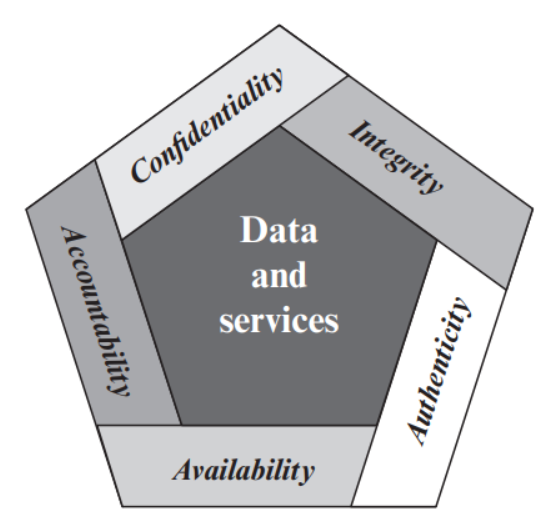
\includegraphics[width=\linewidth]{images/image-security.png}
    \caption{Essential Network and Computer Security Requirements.} \label{fig1}
    \vspace{0.5em}
    \begin{center}
        {\small Źródło: William Stallings, *Cryptography and Network Security*, 7. wydanie.}
    \end{center}
\end{figure}

\subsubsection{Definicja kryterium oceny pod kątem skalowalności}

Czym jest skalowalność

W rozdziale 1 autorzy definiują pojęcie skalowalności jako 4 główne aspekty systemu: Controlling the cost of physical resources, Controlling the performance loss, Preventing software resources running out, Avoiding performance bottlenecks, strony 20-21, czyli Kontrola kosztów zasobów fizycznych, Kontrola utraty wydajności, Zapobieganie wyczerpywaniu się zasobów oprogramowania, Unikanie wąskich gardeł wydajności, dlatego mogę zdefiniować kryterium oceny pod kątem skalowalności jako: ~\cite[p. 21]{coulouris2011distributed}

\begin{enumerate}
    \item Wpływ na koszty zasobów fizycznych - to jak wzrostu obciążenia wpływa na koszty utrzymania sprzętu.
    \item Wpływ na wydajność - wydajność systemu w miarę wzrostu obciążenia.
    \item Wpływ na zasoby serwera - jak program wykorzystuje zasoby serwera w miarę wzrostu obciążenia.
    \item Unikanie wąskich gardeł wydajności - wiarygodność powstania wąskich gardeł w miarę wzrostu obciążenia systemu.
\end{enumerate}

\subsubsection{Definicja kryterium oceny pod kątem wersjonowania}

Za pomocą źródeł literaturowych oraz własnego doświadczenia zdefiniowałem kryteria oceny pod kątem wersjonowania jako:

% AI
\begin{enumerate}
    \item \textbf{Kompatybilność wsteczna} - Zapewnienie, że starsze wersje systemu lub komponentów nadal będą działały poprawnie, mimo wprowadzania nowych wersji. Kompatybilność wsteczna pomaga zapewnić funkcjonowanie istniejących systemów mikroserwisów w trakcie wprowadzania zmian i rozwoju systemu, pozwala przejść z kosztownych i bardzo skomplikowanych upgrade'ów systemu w całości za raz, a podzielić prace na mniejsze, łatwiejsze do zarządzania kawałki.  ~\cite[p. 75]{bloch2018effective}
    \item \textbf{Łatwość migracji} - Prostota przejścia między wersjami, umożliwienie łatwego przechodzenia między różnymi wersjami plików lub interfejsów, aby dostosować się do zmian bez wprowadzania zakłóceń w pracy systemu. Możliwość zmniejszenia przestojów aplikacji w trakcie prac serwisowych i możliwość płynnego przejścia na nową wersję. Proste migracje przyspieszają proces rozwoju aplikacji i zmniejszają ilość błędów. ~\cite[p. 78]{bloch2018effective}
    \item \textbf{Zarządzanie historią wersji} - Możliwość przechowywania i uzyskiwania dostępu do poprzednich wersji plików. Historia wersji pozwala programistom szybko i łatwo przywrócić poprzednią wersję w przypadku powstania błędu w nowej wersji. Pozwala na zmniejszenie utraty danych i niespójności w trakcie rozwoju aplikacji. Posiadanie historii wersji zapewnia to, że projekty pozostają łatwe w utrzymaniu i skalowalne. ~\cite[p. 150]{rubin2012essential}
    \item \textbf{Śledzenie zmian} - Zdolność systemu do rejestrowania i monitorowania wszystkich zmian. Możliwość śledzenia zmian zapewnia to, że każda zmiana w systemie będzie zapisana, wspierając tym programistów w zrozumieniu problemów i błędów albo pozwalając cofnąć zmiany. Poprawia współpracę między zespołami, wykazując kto, kiedy i dlaczego wprowadzał zmiany, co zwiększa również odpowiedzialność. W branżach regulowanych prawem taka audytowalność systemu może być wymagana przez prawo. ~\cite[p. 150]{rubin2012essential}
\end{enumerate}

\subsection{Ocena i porównanie metod współdzielenia kodu}

\subsubsection{Ocena współdzielenia kodu za pomocą Interface definition languages}

Ocena pod kątem komunikacji – zapewnia potrzebny poziom komunikacji, obiekty są generowane na podstawie języka definicji interfejsu (IDL) na etapie uruchamiania aplikacji. Dalej, w trakcie wykonywania logiki programu, takie obiekty mogą być używane przez program bez obciążenia wydajnościowego. Obiekty wygenerowane na podstawie plików IDL mogą być wykorzystane do komunikacji asynchronicznej, takich jak brokery wiadomości, jak również do wysyłania bezpośrednich zapytań między serwisami.

Metody zarządzania plikami idl w systemach :

% AI
\begin{enumerate}
    \item SVN systemy takie jak, na przykład GIT - Rozwiązania posiada następujące korzyści: łatwe osiągnięcie wstecznej kompatybilności, ułatwienie osiągnięcia jednego źródła prawdy w systemie mikroserwisów, łatwiejsze zapewnienie tego, że wszystkie usługi korzystają z najnowszej wersji IDL. Do minusów rozwiązania możemy odnieść to, że system SVN może szybko stać wąskim gardłem w przypadku wykorzystania przez wiele zespołów, wymaga zarządzania i utrzymania.
    \item Dystrybucja za pomocą bibliotek - Kompilowanie plików IDL do współdzielonych bibliotek, i publikacja w współdzielonym repozytorium pakietów, na przykład Nexus. Do korzyści tego rozwiązania możemy odnieść łatwą integrację z procesami CI/CD, możliwość korzystania z wersjonowanych artefaktów bez bezpośredniej interakcji z surowymi plikami IDL oraz to, że różne języki programowania mogą wymagać różnych bibliotek, co zwiększa złożoność systemu.
    \item Podejście Monorepo - Przechowywanie wszystkich mikroserwisów i powiązanych z nimi plików IDL w jednym repozytorium, co zapewni, że wszystkie zespoły będą pracować na tej samej bazie kodu. Do korzyści tego rozwiązania możemy odnieść to, że pliki IDL w implementacjach usług są zawsze zsynchronizowane oraz to, że takie podejście upraszcza zarządzanie zależnościami, ponieważ cały kod przechowywany jest w jednym miejscu. Do wad podejścia mogę odnieść problemy ze skalowalnością, zwiększenie ilości kodu oraz to, że często wymaga narzędzi do zarządzania dużymi bazami kodu.
    \item Repozytoria z automatyczną synchronizacją - Repozytoria z automatyczną synchronizacją to specyficzny rodzaj repozytoriów, w których zmiany wprowadzone w głównym repozytorium są automatycznie propagowane do pozostałych subrepozytoriów. Dzięki temu każdy uczestnik projektu ma dostęp do wszystkich wersji kodu. Do zalet tego podejścia możemy zaliczyć możliwość scentralizowanego wymuszania wersjonowania oraz łatwy dostęp do wszystkich wersji plików. Do minusów możemy zapisać dość trudne utrzymanie oraz złożoność w zarządzaniu synchronizacją i konfliktami w repozytorium.
    \item IDL as a Service (IDLaS) - Przygotowana wcześniej usługa, która obsługuje pliki IDL na żądanie. Ta usługa może wersjonować, weryfikować i dostarczać pliki IDL. Do korzyści tego podejścia możemy odnieść dostęp na żądanie do plików IDL, możliwość dynamicznego wersjonowania. Do minusów możemy doliczyć to, że takie podejście wymaga zbudowania i utrzymania dodatkowej usługi w systemie oraz to, że komunikacja sieciowa może powodować opóźnienia w dostarczaniu plików IDL.
\end{enumerate}

Ocena pod kątem izolacji - ocena pod kątem izolacji zależy od implementacji zarządzania plikami IDL, dla każdego z powyżej opisanego podejścia dokonałem analizy.

Ze względu na to, że mamy wiele kryteriów oceny i wiele możliwych podejść do współdzielenia plików IDL, postanowiłem stworzyć tabelę porównawczą, która pomoże w czytelnym zaprezentowaniu wyników analizy.

Dane do porównania zostały zebrane z źródeł literaturowych. ~\cite{newman2015building} ,  ~\cite{kleppmann2017designing}
% AI 14%
\begin{table}[htbp]
    \centering
    \caption{Porównanie podejść do współdzielenia kodu w systemach mikroserwisów}
    \label{tab:comparison}
    \begin{tabularx}{\textwidth}{|>{\raggedright\arraybackslash}X|>{\raggedright\arraybackslash}X|>{\raggedright\arraybackslash}X|>{\raggedright\arraybackslash}X|>{\raggedright\arraybackslash}X|>{\raggedright\arraybackslash}X|}
    \hline
    \textbf{Kryteria} & \textbf{SVN/Git Systemy} & \textbf{Biblioteki} & \textbf{Podejście Monorepo} & \textbf{Repo z Auto-Synchro.} & \textbf{IDL as a Service (IDLaS)} \\
    \hline
    \textbf{Conflict Rate} &
    Wysoki: Merge konflikty są powszechne w przypadku wykorzystania przez kilkoma zespołami jednocześnie. Rozwiązanie takich konfliktów może być zasobochłonne &
    Umiarkowany: Konflikty są mniej powszechne, ale wciąż mogą wystąpić. &
    Niski: Zespoły pracują na tej samej bazie kodu, dlatego konflikty zdarzają się rzadko, mogą wystąpić w trakcie pracy na tej samej usłudze. &
    Umiarkowany: Konflikty mogą wystąpić, dlatego w przypadku gdy synchronizacja między usługami nie jest dobrze zarządzana. &
    Niski: Konflikty zdarzają się rzadko, dlatego, że IDL są dostarczane na żądanie a wersjonowanie jest wymuszane. \\
    \hline
    \textbf{Version Drift Occurrence} &
    Umiarkowana: Może wystąpić jeśli zespoły programistów nie aktualizują się do nowszej wersji regularnie. &
    Niski: Wiarygodność jest minimalna, ponieważ biblioteki są wersjonowane i dystrybuowane za pomocą odpowiednich narzędzi. &
    Niski: Bazy kodu w tym przypadku baza kodu jest synchronizowana co minimalizuje problemy z wersjonowaniem. &
    Umiarkowany: Problemy mogą wystąpić, jeśli synchronizacja nie jest dobrze utrzymana. &
    Bardzo Niski: Dynamiczne zarządzanie wersjami po stronie usługi zmniejsza wiarygodność problemów z wersjonowaniem. \\
    \hline
    \textbf{Build Failure Rate} &
    Wysoki: Błędy w trakcie kompilacji mogą wystąpić w przypadku niekompatybilnych usług. &
    Umiarkowana: Awarie zdarzają się rzadko, możliwe są z przypadku nieprawidłowych wersji zawartych w bibliotece. &
    Umiarkowana: Błędy w trakcie kompilacji zdarzają się rzadko, ze względu na synchronizację kodu. &
    Umiarkowana: Błędy w trakcie kompilacji zdarzają się rzadko, możliwe w przypadku niedysynchronizacji repozytorium. &
    Niska: Minimalne ryzyko błędów w trakcie kompilacji ze względu na wymuszaną synchronizację. \\
    \hline
    \textbf{Deployment Rollback Frequency} &
    Wysoka: Częste zmiany w plikach IDL mogą spowodować częste wycofanie zmian w trakcie wdrożenia. &
    Umiarkowana: Wycofania zmian w trakcie wdrożenia mogą wystąpić, jeśli wystąpią problemy z kompatybilnością wsteczną. &
    Umiarkowana: Wycofania zmian w trakcie wdrożenia są rzadsze ze względu na synchronizację, ale problemy mogą wystąpić. &
    Niska: Wycofania zmian w trakcie wdrożenia są rzadkie, automatyczna synchronizacja minimalizuje potrzebę wycofywania zmian. &
    Niska: Wycofania zmian w trakcie wdrożenia są rzadkie. Zarządzanie IDL na żądanie zmniejsza częstotliwość wycofywania. \\
    \hline
    \end{tabularx}
\end{table}

\newpage

Ocena pod kątem bezpieczeństwa:
% AI 15%
\begin{longtable}{|p{4cm}|p{4cm}|p{4cm}|}
    \caption{Porównanie SVN, bibliotek, Monorepo i IDLaS pod kątem bezpieczeństwa.} \\
    \hline
    \textbf{Kryteria} & \textbf{Zalety} & \textbf{Wyzwania} \\ \hline
    \multicolumn{3}{|c|}{\textbf{SVN }} \\ \hline
    Poufność & Zaawansowane mechanizmy kontroli dostępu wspierają w zapewnieniu poufności & Wymaga odpowiedniej dodatkowej konfiguracji \\ \hline
    Integralność & Pełna i przejrzysta historia zmian zapewnia integralność danych & Problemy z integralnością mogą wystąpić w przypadku, gdy zmiany nie zostaną prawidłowo zsynchronizowane \\ \hline
    Dostępność & Scentralizowane repozytorium dostępne z wielu lokalizacji & Awaria serwera centralnego może ograniczyć dostęp \\ \hline
    Autentyczność & Uwierzytelnianie użytkowników kontroluje dostęp do repozytorium & Nieprawidłowa konfiguracja uwierzytelniania może prowadzić do problemów z bezpieczeństwem \\ \hline
    Odpowiedzialność & Za pomocą uwierzytelniania można kontrolować dostęp do repozytorium & Proces przeprowadzenia audytu w systemie musi być prawidłowo skonfigurowany \\ \hline
    \multicolumn{3}{|c|}{\textbf{Dystrybucja za pomocą bibliotek (Nexus)}} \\ \hline
    Poufność & Uwierzytelnianie i mechanizmy kontroli dostępu pomagają chronić pliki IDL & Nieprawidłowa konfiguracja może prowadzić do nieautoryzowanego udostępniania \\ \hline
    Integralność & Kontrola wersji artefaktów zapewnia integralność & Brak wersjonowania może spowodować problemy \\ \hline
    Dostępność & Scentralne przechowywanie artefaktów zapewnia dla nich dostępność & Wymaga dodatkowej konfiguracji do prawidłowego działania \\ \hline
    Autentyczność & Mechanizmy podpisywania artefaktów pomagają w znalezieniu zaufanych źródeł & Wymaga prawidłowej konfiguracji \\ \hline
    Odpowiedzialność & Nie wszystkie rozwiązania zapewniają audyt i monitorowanie działań użytkowników & Właściwe logowanie zewnętrzne jest niezbędne do rozliczalności \\ \hline
    \multicolumn{3}{|c|}{\textbf{Podejście Monorepo}} \\ \hline
    Poufność & Scentralizowana kontrola dostępu pomaga poprawić bezpieczeństwo & Zarządzanie dostępem w dużych repozytoriach potrafi być skomplikowane \\ \hline
    Integralność & Scentralizowane zarządzanie zmianami pomaga w zapewnieniu spójności & Są różne wyzwania związane z synchronizacją w dużych zespołach \\ \hline
    Dostępność & Scentralizowane repozytorium umożliwia łatwy dostęp do treści repozytorium & Wymaga solidnie postawionej infrastruktury do użytku na dużą skalę \\ \hline
    Autentyczność & Kontrola dostępu na wyższym poziomie w organizacji pomaga w zapewnieniu bezpieczeństwa & Zarządzanie uprawnieniami w dużych zespołach jest trudne i może doprowadzić do błędów \\ \hline
    Odpowiedzialność & Scentralizowane procesy biznesowe umożliwiają pełne śledzenie zmian & W dużych organizacjach trudniej znaleźć odpowiedzialnego za błąd w rezultacie audytu \\ \hline
    \multicolumn{3}{|c|}{\textbf{IDL as a Service (IDLaS)}} \\ \hline
    Poufność & Bezpieczne punkty końcowe API z uwierzytelnianiem i szyfrowaniem zapewniają poufność & Wymaga konfiguracji bezpieczeństwa i stałego monitorowania dostępu \\ \hline
    Integralność & Systemy kontroli wersji i automatyczna dokumentacja mogą pomóc w zapewnieniu integralności zmian & Nieprawidłowe zarządzanie wersjami może prowadzić do problemów z integralnością \\ \hline
    Dostępność & Zapewnia wysoką dostępność dzięki automatycznemu zarządzaniu zasobami & Zależność od stabilnego połączenia sieciowego \\ \hline
    Autentyczność & Mechanizmy uwierzytelniania, autoryzacji i certyfikatów cyfrowych wspomagają uwierzytelnienie & Wymaga regularnego monitorowania systemu bezpieczeństwa \\ \hline
    Odpowiedzialność & Szczegółowe logi umożliwiają precyzyjne śledzenie zmian & Integracja z systemami zarządzania logami wymaga konfiguracji \\ \hline
\end{longtable}

Ocena pod kątem wersjonowania:

Na podstawie analizy źródeł literaturowych oraz własnych doświadczeń dokonałem analizy podejścia do współdzielenia kodu za pomocą plików IDL. W tym przypadku ocena pod kątem wersjonowania różni się w zależności od przyjętego podejścia do zarządzania plikami IDL, dlatego przeprowadziłem porównanie dla każdego z tych podejść.

\begin{longtable}{|C{3cm}|C{9.1cm}|}
    \caption{Porównanie podejść do zarządzania kodem, wersjonowania i repozytoriami: Git, biblioteki, Monorepo i IDLaS.} \\
    \hline
    \textbf{Zaleta} & \textbf{Opis} \\
    \hline
    \endfirsthead

    \hline
    \textbf{Zaleta} & \textbf{opis} \\
    \hline
    \endhead

    \hline
    \endfoot

    \hline
    \endlastfoot

    \multicolumn{2}{|c|}{\textbf{1. SVN Systemy (Git)}} \\ \hline
    śledzienie zmian &
    \begin{itemize}
      \item Każda zmiana jest rejestrowana w postaci commitu z timestampem i informacjami wskazującymi autora.
      \item Rozgałęzianie i tagowanie umożliwiają izolowane przygotowanie paczki zmian i później oznaczanie stabilnych wersji.
      \item Pełna historia commitów umożliwia przeprowadzani audytów.
    \end{itemize} \\ \hline
    Rozgałęzianie i tagowanie &
    \begin{itemize}
      \item Rozgałęzienie pozwala zespołom na przygotowanie nowych wersji oprogramowania w izolacji, nie przerywając pracy innych zespołów.
      \item Tagi dają możliwości oznaczania stabilnych wersji, zapewniając łatwą identyfikację wersji gotowych do użytku.
    \end{itemize} \\ \hline
    Audytowalność &
    \begin{itemize}
      \item Pełna historia commitów jest zawsze przechowywana, co umożliwia audyty kodu.
      \item Zapewnia odpowiedzialność za wprowadzone zmiany i usprawnia współpracę zespołów.
    \end{itemize} \\ \hline

    \multicolumn{2}{|c|}{\textbf{2. Biblioteki}} \\ \hline
    Wersjonowanie semantyczne &
    \begin{itemize}
      \item Artefaktom przypisywane są numery.
      \item Do każdej wersji dołączone są "Release notes".
      \item Repozytoria przechowują pełną historię wersji.
    \end{itemize} \\ \hline
    Dzienniki zmian &
    \begin{itemize}
      \item Do każdego wydania dołączona szczegółowa dokumentacja.
      \item Takie dzienniki zmian zapewniają uporządkowaną historię modyfikacji.
      \item Takie podejście zapewnia to przejrzystość śledzenia zmian.
    \end{itemize} \\ \hline
    Centralne repozytorium artefaktów &
    \begin{itemize}
      \item Centralne repozytorium przechowuje kompletną historię wersji.
      \item Dzięki temu zespoły mogą, w razie potrzeby, pobierać, porównywać i przywracać wcześniejsze stabilne wersje.
    \end{itemize} \\ \hline

    \multicolumn{2}{|c|}{\textbf{3. Podejście Monorepo}} \\ \hline
    Zunifikowany dziennik zmian &
    \begin{itemize}
      \item Wszystkie mikroserwisy w systemie i powiązane z nimi pliki IDL znajdują się w jednym repozytorium.
      \item Historia commitów zapewnia całościowy widok zmian.
    \end{itemize} \\ \hline
    Spójność &
    \begin{itemize}
      \item Wszystkie zmiany są wprowadzane do jednego repozytorium, co zapewnia synchronizację.
      \item Takie podejście minimalizuje ryzyko różnic w wersjach pomiędzy usługami.
      \item Spójne wersjonowanie poprawia stabilność systemu.
    \end{itemize} \\ \hline
    Łatwość cofanięcia &
    \begin{itemize}
      \item Scentralizowana historia ułatwia powrót do poprzedniego stabilnego stanu.
      \item Takie podejście ułatwia debugowanie i zwiększa stabilność systemu.
    \end{itemize} \\ \hline

    \multicolumn{2}{|c|}{\textbf{4. IDL as a Service (IDLaS)}} \\ \hline
    Zintegrowana kontrola wersji &
    \begin{itemize}
      \item Dostarczana usługa obejmuje wbudowaną kontrolę wersji.
      \item Dostarczana usługa daje dostęp do historii wersji za pomocą API.
    \end{itemize} \\ \hline
    Automatyczna dokumentacja &
    \begin{itemize}
      \item IDLaS często udostępniają interfejsy webowe.
      \item Ze względu na to, że IDL jest udostępniane jako usługa, każdy użytkownik może uzyskać dostęp do historii wersji za pomocą API.
    \end{itemize} \\ \hline

\end{longtable}

\subsubsection{Ocena współdzielenia kodu za pomocą bibliotek}

Ocena pod kątem komunikacji:

Pod kątem komunikacji podejście zapewnia potrzebny poziom komunikacji, obiekty są dodawane do projektu przez narzędzie do budowania projektów na etapie uruchamiania aplikacji, dalej w trakcie wykonania logiki programu takie obiekty mogą być użyte przez program bez żadnych obciążeń wydajnościowych. Obiekty wciągnięte z biblioteki mogą być użyte dla komunikacji asynchronicznej, takich jak brokery wiadomości, jak również dla wysłania bezpośrednich zapytań między serwisami.

Ocena pod kątem izolacji:

Zgodnie z wcześniej zaprezentowanymi kryteriami oceny, w przypadku oceny izolacji bibliotek, kryteria oceny są następujące: ocena pod kątem izolacji interfejsów, izolacji wersji oraz izolacji zależności.

Izolacja interfejsów: Dobrze ustrukturyzowana biblioteka izoluje skomplikowane elementy logiki od swoich użytkowników. Gdy są użyte prawidłowo, biblioteki pozwalają na zmianę lub aktualizację kodu przy minimalnym wpływie na kod wykorzystujący bibliotekę.  ~\cite[p. 75]{Essential}

Izolacja wersji: Biblioteki zazwyczaj używają semantycznego wersjonowania za pomocą nazwy. Przejrzysta historia wersji umożliwia deweloperom odpowiednie zarządzanie zależnościami. Przy odpowiedniej izolacji wersji wiele wersji biblioteki może współistnieć i być używane jednocześnie, ułatwia to proces stopniowej migracji. ~\cite[p. 172]{fowler2012patterns}

Izolacja zależności: Biblioteki często zależą od innych bibliotek, w przypadku gdy zależności nie są prawidłowo izolowane mogą prowadzić do konfliktów i innych problemów. Dobre praktyki zarządzania zależnościami pomagają zapewnić, że zależności biblioteki nie będą miały negatywnego wpływu na aplikację. ~\cite[p. 218]{martin2008clean}

Ocena pod kątem bezpieczeństwa:

Zgodnie z wcześniej zaprezentowanymi kryteriami oceny, w przypadku oceny bezpieczeństwa bibliotek kryteria oceny są następujące: Poufność, Integralność danych, Dostępność, Autentyczność, Odpowiedzialność.

Poufność: Biblioteki, które są wykorzystywane do przetwarzania poufnych danych muszą pochodzić z sprawdzonych źródeł i ciągle aktualizowane, aby zapobiec utracie danych. ~\cite[p. 82]{Essential}

Integralność danych: Biblioteki często korzystają z sum kontrolnych, certyfikatów, podpisów cyfrowych aby mieć pewność, że przetwarzane dane pozostają bezpieczne. ~\cite[p. 84]{Essential}

Dostępność: Dostępność może zostać naruszona, jeśli biblioteki zewnętrzne będą niedostępne, lub wewnętrzne w przypadku awarii narzędzia do zarządzania bibliotekami. Dlatego ważne jest wykorzystanie menedżerów zależności które są zaufane. ~\cite[p. 85]{Essential}

Autentyczność: W przypadku bibliotek jest zapewniana za pomocą sprawdzenia jej pochodzenia za pomocą podpisów cyfrowych i sum kontrolnych dostarczonych przez wydawcę. Zapobiega to ryzyku włączenia wykonania złośliwego kodu po stronie klienta biblioteki.  ~\cite[p. 87]{Essential}

Odpowiedzialność: W przypadku bibliotek przejrzysta historia może zostać zapewniona za pomocą menedżerów pakietów, które umożliwiają śledzenie pochodzenia zmian. Wspomaga to w zapewnieniu odpowiedzialności w przypadku problemów.  ~\cite[p. 88]{Essential}

\subsubsection{Ocena współdzielenia kodu za pomocą SDK}

Ocena pod kątem komunikacji: zapewnia potrzebny poziom komunikacji, mechanizm współdzielenia jest podobny do biblioteki, tak samo jak w przypadku biblioteki obiekty są dodawane do projektu przez narzędzie do budowania projektów na etapie uruchamiania aplikacji, dalej w trakcie wykonania logiki programu takie obiekty mogą być użyte przez program bez żadnych obciążeń wydajnościowych. Obiekty wciągnięte z biblioteki mogą być użyte dla komunikacji asynchronicznej takich jak brokery wiadomości jak również dla wysłania bezpośrednich zapytań między serwisami.

Ocena pod kątem izolacji:

Zgodnie z wcześniej zaprezentowanymi kryteriami oceny, w przypadku oceny izolacji SDK kryteria oceny są następujące: ocena pod kątem izolacji interfejsów, izolacja wersji, izolacja zależności. Jednak są one trudniejsze w projektowaniu i wymagają ostrożności w trakcie zarządzania. ~\cite[p. 75]{EssentialIan}

Izolacja wersji: W przypadku SDK, które agregują kilka bibliotek i narzędzi, muszą zarządzać wersjonowaniem wszystkich zawartych komponentów. W idealnym przypadku zestaw SDK jest zaprojektowany tak, aby nowe dodane wersje były kompatybilne wstecz, umożliwiając klientom działanie bez natychmiastowych zmian.

Izolacja zależności: SDK często zawierają wiele bibliotek w sposób, co oznacza, że często zarządzają dużą ilością zależności. Izolowanie tych zależności jest krytyczne, aby uniknąć konfliktów. ~\cite[p. 218]{martin2008clean}

% AI
Ocena pod kątem bezpieczeństwa:

Zgodnie z wcześniej zaprezentowanymi kryteriami oceny, w przypadku oceny bezpieczeństwa bibliotek kryteria oceny są następujące: Poufność, Integralność danych, Dostępność, Autentyczność, Odpowiedzialność

Poufność: SDK muszą zapewnić, że wszystkie zawarte komponenty przestrzegają ścisłych zasad kontroli dostępu zmniejszając to ryzyko nieautoryzowanego dostępu do danych.  ~\cite[para 4]{azure2020}

Integralność danych: SDK wymaga, aby były one kompleksowo testowane, aby zapewnić, że zmiany nie naruszą integralności danych. Różne frameworki do testowania bezpieczeństwa SDK pomagają w wykrywaniu wszelkich podatności po modyfikacji.  ~\cite[para 5]{azure2020}

Dostępność: SDK muszą być zaprojektowane tak, aby działały zawsze, nawet przy dużym obciążeniu. ~\cite[para 6]{azure2020}

Autentyczność: Autentyczność w przypadku SDK może zostać zapewniona za pomocą weryfikacji dostawców i stosowania środków kryptograficznych do walidacji ich komponentów. Warto dokonywać takich działań, aby zapobiec wykonaniu złośliwego kodu w naszym systemie. ~\cite[para 7]{azure2020}

Odpowiedzialność: SDK zazwyczaj posiadają różne mechanizmy zarządzania wersjami. Takie metody zarządzania wersjami umożliwiają deweloperom śledzenie pochodzenia wszelkich zmian lub problemów. Pomaga to zapewnić odpowiedzialność programistów za przygotowane zmiany. ~\cite[para 7]{azure2020}

Ocena pod kątem wersjonowania:

SDK mogą zawierać wiele bibliotek i narzędzi, z których każde może mieć własną historię wersji. Wersjonowanie SDK potrafi być złożone, ponieważ musimy uwzględniać zmiany we wszystkich wewnętrznych komponentach, prowadzi to do bardziej złożonej historii wersji, która wymaga dobrej dokumentacji. ~\cite[para. 3]{azure2020}

Przywracanie kodu do stabilnej wersji: Wycofywanie zmian w przypadku SDK może być trudne, ponieważ SDK może integrować wiele komponentów. Ta złożoność może sprawić, że wycofywanie jest bardziej czasochłonne i podatne na błędy, jeśli nie jest zarządzane prawidłowo. ~\cite[para. 3]{azure2020}

Utrata danych i niespójność: SDK są narażone na większe ryzyko wewnętrznych niespójności i problemów w przypadku, gdy moduły są aktualizowane asynchronicznie. Może to doprowadzić do błędów, które mogą spowodować utratę danych lub uszkodzenie danych, jeśli nie są w odpowiedni sposób zarządzane. ~\cite[para. 3]{azure2020}
%Ai
\subsubsection{Ocena współdzielenia kodu za pomocą API}

Ocena pod kątem komunikacji:

Too podejście zapewnia podstawowy poziom komunikacji poprzez standardowy protokół HTTP/HTTPS.Opiera się na wywoływaniu endpointów API poprzez żądania HTTP. Komunikacja odbywa się poprzez wymianę dokumentów JSON/XML między serwisami, możliwe są zarówno wywołania synchroniczne (bezpośrednie żądania) jak i asynchroniczne. Wymaga dodatkowej konfiguracji i obsługi serializacji/deserializacji danych.

Ocena pod kątem izolacji:

Zgodnie z wcześniej zaprezentowanymi kryteriami oceny, w przypadku oceny izolacji REST kryteria oceny są następujące: ocena pod kątem izolacji interfejsów, izolacja wersji, izolacja zależności.

Izolacja interfejsów: REST API zapewnia jasno zdefiniowane punkty końcowe i kontrakty. Interfejsy są wersjonowane poprzez URL lub nagłówki HTTP, zmiana implementacji wewnętrznej nie wpływa na kontrakt API. Wymagane jest dokładne dokumentowanie API (np. poprzez Swagger/OpenAPI). ~\cite[p. 124]{richardson2013rest}

Izolacja wersji:

Możliwość utrzymywania wielu wersji API równolegle. Wersjonowanie może być realizowane poprzez URL (np. /api/v1/, /api/v2/). Konieczność obsługi kompatybilności wstecznej między wersjami. Złożoność zarządzania rośnie z każdą nową wersją API. ~\cite[p. 89]{richardson2013rest}\

Izolacja zależności:

Serwisy są luźno powiązane, komunikują się tylko poprzez zdefiniowane interfejsy REST. Każdy serwis może być rozwijany i wdrażany niezależnie. Wymagane jest zarządzanie dostępnością i odpornością na błędy. ~\cite[p. 156]{newman2015building}

Ocena pod kątem bezpieczeństwa:

Zgodnie z wcześniej zaprezentowanymi kryteriami oceny, w przypadku oceny bezpieczeństwa REST API kryteria oceny są następujące: Poufność, Integralność danych, Dostępność, Autentyczność, Odpowiedzialność.

Poufność:

Konieczność implementacji mechanizmów autentykacji (np. JWT, OAuth). Wymagane szyfrowanie komunikacji poprzez HTTPS. Możliwość definiowania różnych poziomów dostępu do zasobów. ~\cite[p. 245]{newman2015building}

Integralność danych:

Walidacja danych wejściowych na poziomie API. Konieczność weryfikacji poprawności przesyłanych danych. Możliwość zastosowania podpisów cyfrowych dla krytycznych operacji. ~\cite[p. 267]{newman2015building}

Dostępność:

Konieczność implementacji mechanizmów retry i circuit breaker. Wymagane monitorowanie dostępności usług. Możliwość skalowania poziomego dla zwiększenia dostępności. ~\cite[p. 178]{richardson2013rest}

Autentyczność:

Implementacja mechanizmów uwierzytelniania i autoryzacji. Możliwość wykorzystania certyfikatów SSL/TLS. Konieczność weryfikacji źródła żądań. ~\cite[p. 289]{newman2015building}

Odpowiedzialność:

Możliwość śledzenia wszystkich operacji poprzez logi. Konieczność implementacji mechanizmów audytu. Identyfikacja źródła każdego żądania. ~\cite[p. 312]{newman2015building}

Ocena pod kątem wersjonowania:

REST API wymaga precyzyjnego zarządzania wersjami interfejsów. Konieczność utrzymywania kompatybilności wstecznej. Możliwość równoległego działania wielu wersji API. Wymagane jasne zasady deprecjacji starych wersji. Dokumentacja zmian między wersjami musi być dokładna i aktualna. ~\cite[p. 134]{richardson2013rest}
%AI
\subsubsection{Ocena współdzielenia kodu za pomocą ServerLess}

Ocena pod kątem komunikacji:

Zapewnia wysoki poziom komunikacji poprzez zdarzenia (events) i wywołania funkcji. Mechanizm współdzielenia opiera się na wywoływaniu funkcji bezserwerowych poprzez różne wyzwalacze (triggers), takie jak żądania HTTP, kolejki wiadomości, czy harmonogramy czasowe. Komunikacja odbywa się poprzez przekazywanie zdarzeń i danych między funkcjami, które są automatycznie skalowane w zależności od obciążenia. ~\cite[p. 45]{roberts2018cloud}

Ocena pod kątem izolacji:

Zgodnie z wcześniej zaprezentowanymi kryteriami oceny, w przypadku oceny izolacji architektury serverless kryteria oceny są następujące: ocena pod kątem izolacji interfejsów, izolacja wersji, izolacja zależności.

Izolacja interfejsów:

Funkcje serverless są naturalnie izolowane, każda funkcja posiada własny, jasno zdefiniowany interfejs wejścia/wyjścia. Interfejsy są definiowane poprzez konfigurację zdarzeń i wyzwalaczy. Zmiana implementacji jednej funkcji nie wpływa na inne, o ile zachowany jest kontrakt interfejsu. ~\cite[p. 78]{roberts2018cloud}

Izolacja wersji:
Platformy serverless oferują wbudowane mechanizmy wersjonowania funkcji. Możliwe jest równoległe uruchamianie różnych wersji tej samej funkcji, co ułatwia wdrażanie zmian i testowanie. System aliasów i etapów (stages) pozwala na kontrolowane przełączanie między wersjami. ~\cite[p. 112]{roberts2018cloud}

Izolacja zależności:

Każda funkcja serverless jest całkowicie niezależna i może mieć własne zależności. Pakiety i biblioteki są izolowane na poziomie funkcji, co eliminuje konflikty zależności. Wymaga to jednak zarządzania duplikacją kodu i zależności między funkcjami. ~\cite[p. 156]{roberts2018cloud}

Ocena pod kątem bezpieczeństwa:

Zgodnie z wcześniej zaprezentowanymi kryteriami oceny, w przypadku oceny bezpieczeństwa architektury serverless kryteria oceny są następujące: Poufność, Integralność danych, Dostępność, Autentyczność, Odpowiedzialność.

Poufność:

Platformy serverless zapewniają wbudowane mechanizmy bezpieczeństwa i izolacji. Każda funkcja działa w izolowanym środowisku (sandbox). Dostęp do zasobów jest kontrolowany przez system uprawnień i ról. ~\cite[p. 167]{roberts2018cloud}

Integralność danych:

Funkcje serverless mogą wykorzystywać wbudowane mechanizmy walidacji i transformacji danych. Platformy oferują narzędzia do monitorowania i logowania wszystkich operacji. Możliwe jest wykorzystanie managed services do przechowywania i przetwarzania danych. ~\cite[p. 189]{roberts2018cloud}

Dostępność:

Architektura serverless zapewnia automatyczne skalowanie i wysoką dostępność. Platformy zarządzają infrastrukturą i gwarantują określony poziom SLA. Funkcje są automatycznie replikowane w różnych strefach dostępności. ~\cite[p. 198]{roberts2018cloud}

Autentyczność:

Platformy serverless oferują wbudowane mechanizmy uwierzytelniania i autoryzacji. Możliwa jest integracja z różnymi dostawcami tożsamości. Każde wywołanie funkcji może być weryfikowane pod kątem uprawnień. ~\cite[p. 223]{roberts2018cloud}

Odpowiedzialność:

Platformy zapewniają szczegółowe logowanie i monitorowanie wszystkich wywołań funkcji. Dostępne są narzędzia do analizy wydajności i kosztów. Możliwe jest śledzenie całego łańcucha wywołań między funkcjami. ~\cite[p. 245]{roberts2018cloud}

Ocena pod kątem wersjonowania:

Wersjonowanie w architekturze serverless jest wspierane przez wbudowane mechanizmy platform. Każda funkcja może mieć wiele wersji, które są zarządzane niezależnie. System aliasów pozwala na kierowanie ruchu do określonych wersji funkcji. Możliwe jest stopniowe wdrażanie zmian poprzez techniki takie jak canary deployments. ~\cite[p. 267]{roberts2018cloud}

Przywracanie kodu do stabilnej wersji:

W przypadku problemów możliwe jest szybkie przełączenie na poprzednią stabilną wersję funkcji. Platformy serverless przechowują historię wersji i umożliwiają łatwe przełączanie między nimi. ~\cite[p. 289]{roberts2018cloud}

Utrata danych i niespójność:

Ryzyko utraty danych jest minimalizowane przez wykorzystanie managed services do przechowywania stanu. Transakcyjność może być zapewniona przez odpowiednie projektowanie przepływu danych między funkcjami. ~\cite[p. 312]{roberts2018cloud}

\newpage
% new
\subsubsection{Ocena współdzielenia pod kątem skalowalności}

Ocena podejścia IDL pod kątem skalowalności:

Systemy bazujące na IDL, takie jak Protocol Buffers oraz Avro zazwyczaj serializują dane do kompaktowych formatów binarnych, to znaczy, że ilość danych, które trzeba przesłać przez sieć i przechowywać na dysku, jest minimalna. Dzięki temu koszt zasobów fizycznych jest minimalny i ma tendencję do pozostania niskim, nawet w przypadku wzrostu obciążenia. Wydajność systemu korzystającego z współdzielenia za pomocą IDL nie zależy od metody zarządzania plikami IDL, jak w powyższych przypadkach.

% idl
W celu przygotowania analizy pod kątem skalowalności, opracowałem system, którego celem jest testowanie wydajności przykładowej aplikacji wykorzystującej podejście IDL do współdzielenia kodu oraz obserwacja, w jaki sposób to podejście wpływa na wydajność i skalowalność systemu.

Przygotowane aplikacje przykładowe oraz kod systemu, który powstał w celu sprawdzenia i porównania wydajności, zostały dołączone do materiałów pracy.

Testowany system mikroserwisów składa się z dwóch mikroserwisów napisanych z użyciem technologii Java oraz Spring. Pierwszy mikroserwis produkuje dane, drugi je konsumuje. Oba serwisy uruchamiane są za pomocą narzędzia Docker. Kontenery Dockera mają ustawione limity zasobów, które mogą wykorzystywać.

Po uruchomieniu aplikacji w Dockerze, automatycznie uruchamiane są testy wydajnościowe przygotowane za pomocą narzędzia Gatling. Projekt został stworzony przy użyciu Javy, Springa oraz Gatlinga i znajduje się w materiałach dołączonych do pracy.

W trakcie testów wydajnościowych zbierane są metryki dotyczące użycia pamięci, liczby wątków, zużycia CPU, garbage collection i inne. Dane te są zapisywane do pliku za pomocą narzędzia Java Flight Recorder. Uruchomienie JFR odbywa się również automatycznie w momencie startu aplikacji za pomocą skryptu, kod skryptu również znajduje się w materiałach dołączonych do pracy.

Aplikacja testująca wydajność aplikacji przykładowej posiada trzy tryby testowania: małe obciążenie, średnie oraz duże. Zostało to zrealizowane w celu obserwacji działania aplikacji przy różnych poziomach obciążenia.

\newpage

\begin{figure}
    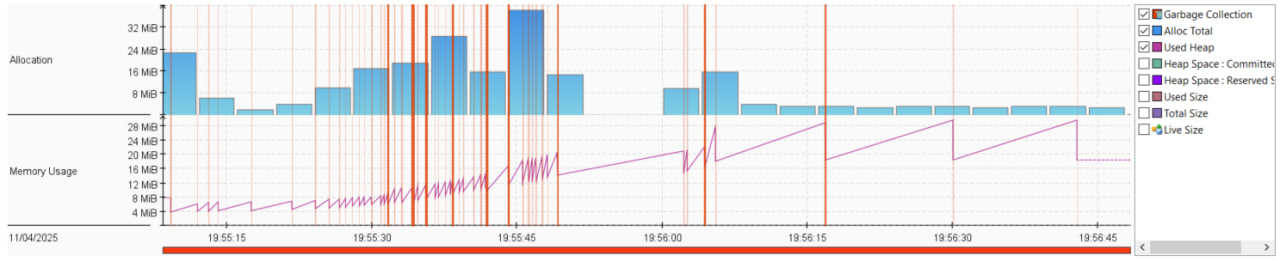
\includegraphics[width=\linewidth]{images/idl-memory-low-graph.jpg}
    \caption{Wykres przedstawiający zużycie pamięci RAM aplikacji wykorzystującej podejście IDL pod wpływem małego obciążenia.} \label{fig1}
    \vspace{0.5em}
    {\small Źródło: opracowanie własne.}
\end{figure}

% idl memory descriptiuon
Wyniki obserwacji:

Alokacja (górny wykres — niebieskie słupki)

\begin{itemize}
    \item Szczyty alokacji są bardziej okresowe i zazwyczaj utrzymują się poniżej 32~MiB.
    \item Występuje więcej przerw między zdarzeniami alokacji, co wskazuje na rzadsze tworzenie nowych obiektów.
\end{itemize}

Garbage collection (pionowe pomarańczowe linie)

\begin{itemize}
    \item Ogólnie mniej zdarzeń GC.
    \item GC wydaje się być wyzwalane rzadziej ze względu na mniejsze obciążenie pamięci.
\end{itemize}

Wykorzystanie pamięci (dolny wykres – fioletowa linia)

\begin{itemize}
  \item Wykorzystanie sterty rośnie powoli i konsekwentnie, osiągając maksymalnie około 24~MiB.
  \item Stopniowy wzrost z regularnymi małymi spadkami (GC), pokazujący stabilne wykorzystanie pamięci.
\end{itemize}

\newpage

\begin{figure}
    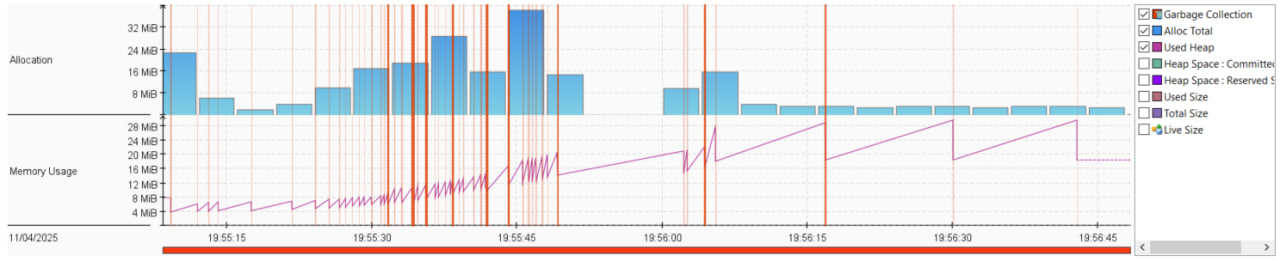
\includegraphics[width=\linewidth]{images/idl-memory-low-graph.jpg}
    \caption{Wykres przedstawiający zużycie pamięci RAM aplikacji wykorzystującej podejście IDL pod wpływem średniego obciążenia.} \label{fig1}
    \vspace{0.5em}
    {\small Źródło: opracowanie własne.}
\end{figure}

Wyniki obserwacji:

Alokacja (górny wykres — niebieskie słupki)

\begin{itemize}
  \item Aktywność alokacji jest większa i bardziej spójna.
  \item Maksymalne wartości osiągają 48~MiB, co wskazuje na znaczny wzrost alokacji obiektów ze względu na większą liczbę żądań.
  \item Alokacje są utrzymywane przez dłuższy okres z krótszym czasem bezczynności między słupkami.
\end{itemize}

Garbage collection (pionowe pomarańczowe linie)

\begin{itemize}
  \item Znacznie częstsze zdarzenia GC.
  \item Wskazuje na zwiększoną utratę pamięci — częstsze tworzenie i czyszczenie obiektów ze względu na dużą liczbę żądań.
\end{itemize}

Wykorzystanie pamięci (dolny wykres – fioletowa linia)

\begin{itemize}
  \item Wykorzystanie sterty wzrasta do 64~MiB i okresowo spada.
  \item Wzór pokazuje częste cykle alokacji i GC, sugerując agresywne wykorzystanie pamięci i czyszczenie.
\end{itemize}

<<<<<<< HEAD
W przypadku dużego obciążenia nie miałem możliwości wygenerowania raportu ze względu na błąd pamięci (Memory Error).
=======
W przypadku dużego obciążenia nie miałem możliwości wygenerować raport ze względu na Memory Error.
>>>>>>> 64966de36be71826c93c5c7934c9ca0fa456c72c

\newpage

% idl gatling descrition

Raporty wygenerowane przez narzędzie Gatling:

\begin{figure}
    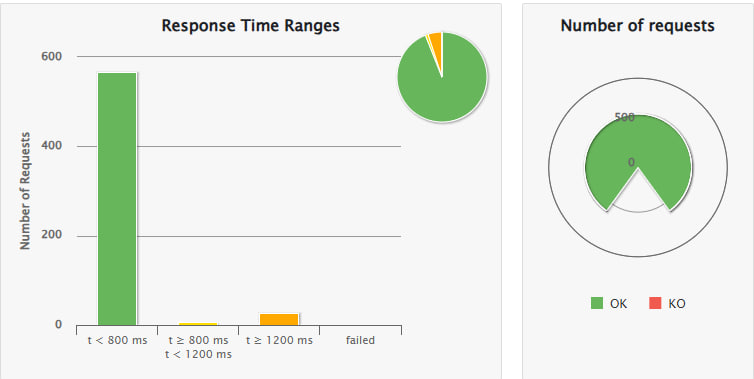
\includegraphics[width=\linewidth]{images/idl-low-gatling-graph.jpg}
    \caption{Raport wygenerowany w narzędziu Gatling dla aplikacji działającej w oparciu o podejście IDL, testowanej przy niskim obciążeniu.} \label{fig1}
    \vspace{0.5em}
    {\small Źródło: opracowanie własne.}
\end{figure}

Na rysunku widać, że:

\begin{itemize}
    \item Czas odpowiedzi krótszy niż 800 ms: Zdecydowana większość żądań (około 580), oznaczona kolorem zielonym.
    \item Czas odpowiedzi od 800 ms do poniżej 1200 ms: Niewielka liczba żądań, przedstawiona kolorem żółtym.
    \item Czas odpowiedzi równy lub przekraczający 1200 ms: Również niewielka liczba żądań.
    \item Żądania nieudane: Brak nieudanych żądań.
\end{itemize}

\newpage

\begin{figure}
    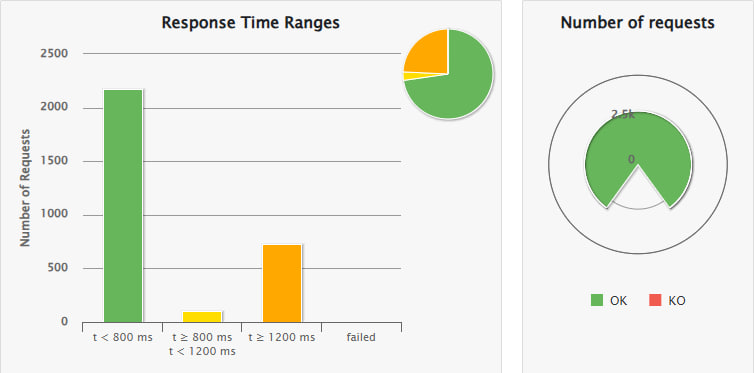
\includegraphics[width=\linewidth]{images/idl-midle-gatling-graph.jpg}
    \caption{Raport wygenerowany w narzędziu Gatling dla aplikacji działającej w oparciu o podejście IDL, testowanej przy średnim obciążeniu.} \label{fig1}
    \vspace{0.5em}
    {\small Źródło: opracowanie własne.}
\end{figure}

<<<<<<< HEAD
Na rysunku zaobserwowałem:
=======
Na rysunku zaobsewowałem:
>>>>>>> 64966de36be71826c93c5c7934c9ca0fa456c72c

\begin{itemize}
    \item Czas odpowiedzi krótszy niż 800 ms: Duża liczba żądań (około 2300), jednak proporcjonalnie mniej niż w przypadku niskiego obciążenia.
    \item Czas odpowiedzi od 800 ms do poniżej 1200 ms: Niewielki wzrost liczby żądań w porównaniu do niskiego obciążenia.
    \item Czas odpowiedzi równy lub przekraczający 1200 ms: Wyraźny wzrost – znacznie więcej żądań z długim czasem odpowiedzi.
    \item Żądania nieudane: Nadal brak nieudanych żądań.
\end{itemize}

<<<<<<< HEAD
Na wykresach przedstawionych na podstawie przeprowadzonych testów widać, że zarówno w przypadku małego, jak i średniego obciążenia aplikacja zachowuje się stabilnie. Jednak przy średnim obciążeniu zauważyłem nieznaczne wydłużenie czasu oczekiwania na odpowiedź.

\newpage

Przeprowadzone przeze mnie testy pokazują, że wraz ze zwiększaniem obciążenia wzrasta czas oczekiwania na odpowiedź. Porównując czas oczekiwania w przypadku różnych podejść do współdzielenia kodu, możemy ocenić ich efektywność.
=======
Na przedstawionych na podstawie przeprowadzonych testów wykresach widać, że zarówno w przypadku małego, jak i średniego obciążenia aplikacja zachowuje się stabilnie. Jednak przy średnim zauważyłem nieznaczne wydłużenie czasu oczekiwania na odpowiedź.

\newpage

Przeprowadzone przeze mnie testy pokazują, że zwiększaniem obciążenia wzrasta czas oczekiwania na odpowiedź. Porównując czas oczekiwania w przypadku różnych podejść do współdzielenia kodu, możemy ocenić ich efektywność.
>>>>>>> 64966de36be71826c93c5c7934c9ca0fa456c72c

%sdk
Ocena współdzielenia kodu za pomocą SDK pod kątem skalowalności:

W celu przygotowania analizy pod kątem skalowalności, tak samo jak w poprzednim przypadku opracowałem system, którego celem jest testowanie wydajności przykładowej aplikacji wykorzystującej SDK do współdzielenia kodu oraz obserwacja, w jaki sposób to podejście wpływa na wydajność i skalowalność systemu.

Przygotowane aplikacje przykładowe oraz kod systemu, który powstał w celu sprawdzenia i porównania wydajności, zostały dołączone do materiałów pracy.

Testowany system mikroserwisów składa się z dwóch mikroserwisów napisanych z użyciem technologii Java oraz Spring. Pierwszy mikroserwis produkuje dane, drugi je konsumuje. Oba serwisy uruchamiane są za pomocą narzędzia Docker. Kontenery Dockera mają ustawione limity zasobów, które mogą wykorzystywać.

Po uruchomieniu aplikacji w Dockerze, automatycznie uruchamiane są testy wydajnościowe przygotowane za pomocą narzędzia Gatling. Projekt został stworzony przy użyciu Javy, Springa oraz Gatlinga i znajduje się w materiałach dołączonych do pracy.

W trakcie testów wydajnościowych zbierane są metryki dotyczące użycia pamięci, liczby wątków, zużycia CPU, garbage collection i inne. Dane te są zapisywane do pliku za pomocą narzędzia Java Flight Recorder. Uruchomienie JFR odbywa się również automatycznie w momencie startu aplikacji.

Aplikacja testująca wydajność aplikacji przykładowej posiada trzy tryby testowania: małe obciążenie, średnie oraz duże. Zostało to zrealizowane w celu obserwacji działania aplikacji przy różnych poziomach obciążenia.

\newpage

%sdk memory description

\begin{figure}
    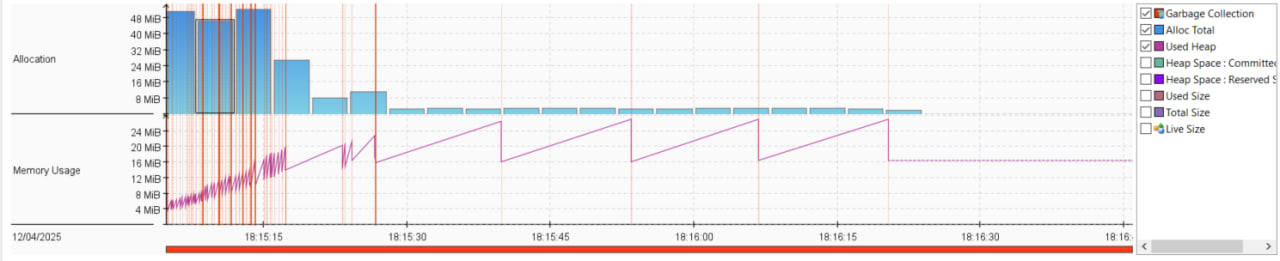
\includegraphics[width=\linewidth]{images/sdk-memory-low-graph.jpg}
    \caption{Wykres przedstawiający zużycie pamięci  RAM aplikacji wykorzystującej SDK pod wpływem małego obciążenia.} \label{fig1}
    \vspace{0.5em}
    {\small Źródło: opracowanie własne.}
\end{figure}

Wyniki obserwacji:

\begin{itemize}
    \item Przegląd: Ten wykres pokazuje stabilny i stosunkowo niski poziom zużycia pamięci.
    \item Wykorzystanie pamięci: Wykorzystanie pamięci osiąga szczyt na poziomie około 200 MB, przy średnim wykorzystaniu około 150 MB. Wykorzystanie pozostaje stale poniżej 250 MB, z niewielkimi skokami dochodzącymi do 220 MB.
    \item Garbage collection: Wykres wskazuje 2-3 zdarzenia zbierania śmieci w całym okresie monitorowania, oznaczone rzadkimi fioletowymi liniami. Sugeruje to wydajne zarządzanie zasobami, ponieważ aplikacja nie wykorzystuje ich intensywnie.
\end{itemize}

\newpage

\begin{figure}
    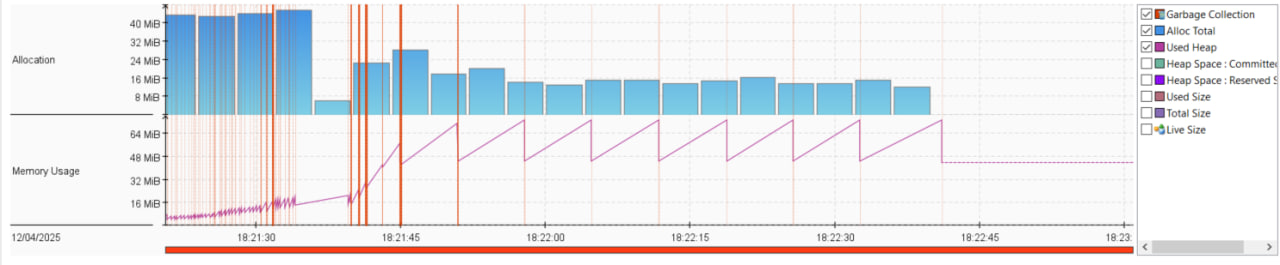
\includegraphics[width=\linewidth]{images/sdk-memory-middle-graph.jpg}
    \caption{Wykres przedstawiający zużycie pamięci  RAM aplikacji wykorzystującej SDK pod wpływem średniego obciążenia.} \label{fig1}
    \vspace{0.5em}
    {\small Źródło: opracowanie własne.}
\end{figure}

\begin{itemize}
    \item Przegląd: Ten wykres przedstawia znaczny wzrost zużycia pamięci w miarę wzrostu obciążenia aplikacji.
    \item Wykorzystanie pamięci: Wykorzystanie pamięci osiąga szczyt na poziomie około 600 MB, przy średnim wykorzystaniu około 450 MB. Wykorzystanie często przekracza 500 MB w godzinach szczytu, ilustrując reakcję aplikacji na większe zapotrzebowanie.
    \item Garbage collection: Wykres pokazuje około 5-7 zdarzeń zbierania śmieci, oznaczonych bardziej wyraźnymi fioletowymi liniami, odzwierciedlającymi potrzebę aplikacji aktywnego zarządzania pamięcią przy zwiększonym obciążeniu.
\end{itemize}

W przypadku dużego obciążenia nie było możliwe wygenerowanie raportu ze względu na Memory Error.
%AI
<<<<<<< HEAD
Wykres, który przygotowałem pod wpływem niskiego obciążenia, sugeruje optymalną wydajność przy minimalnym zużyciu zasobów. Wykres dla średniego obciążenia, pokazujący wyższe zużycie pamięci, wskazuje, że aplikacja skaluje się, aby przetwarzać większą liczbę żądań.
=======
Wykres który przygotowałem pod wpłułem niskeigo obciążenia sugeruje optymalną wydajność przy minimalnym obciążeniu zasobów. Wykres średniego obciążenia, pokazujący wyższe zużycie pamięci, wskazuje, że aplikacja skaluje się, aby przeprocesować większą ilość rządań.

>>>>>>> 64966de36be71826c93c5c7934c9ca0fa456c72c
\newpage

%sdk gatling description

Raporty wygenerowane przez narzędzie Gatling:

\begin{figure}
    \centering
    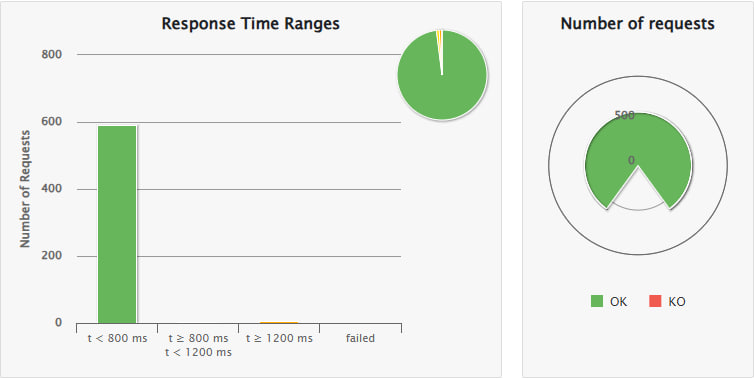
\includegraphics[width=0.8\linewidth]{images/sdk-gatling-low-graph.jpg}
    \caption{Raport wygenerowany w narzędziu Gatling dla aplikacji działającej w oparciu o podejście SDK, testowanej przy niskim obciążeniu.}
    \label{fig:low}
    \vspace{0.5em}
    {\small Źródło: opracowanie własne.}
\end{figure}

\begin{itemize}
    \item Czas reakcji poniżej 800 ms: Około 600 żądań – bardzo dobra wydajność, większość operacji wykonywana szybko.
    \item Czas reakcji od 800 ms do poniżej 1200 ms: Pojedyncze żądania – praktycznie brak wpływu na ogólną wydajność.
    \item Czas reakcji 1200 ms i więcej: Kilka żądań – sporadyczne opóźnienia, nieistotne z punktu widzenia użytkownika.
    \item Nieudane żądania: Brak – aplikacja działa niezawodnie.
\end{itemize}

\newpage

\begin{figure}
    \centering
    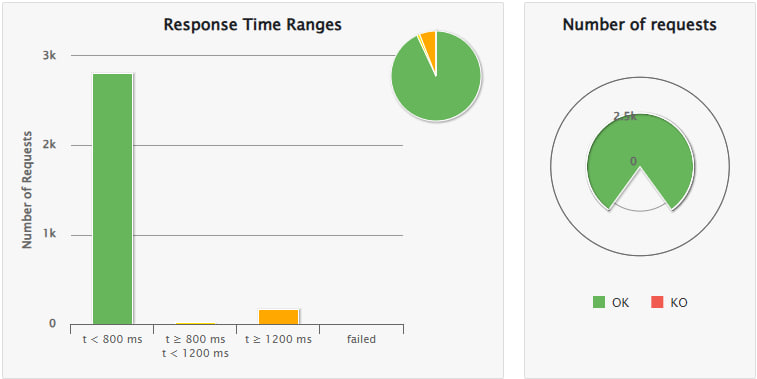
\includegraphics[width=0.8\linewidth]{images/sdk-gatling-middle-graph.jpg}
    \caption{Raport wygenerowany w narzędziu Gatling dla aplikacji działającej w oparciu o podejście SDK, testowanej przy średnim obciążeniu.}
    \label{fig:middle}
    \vspace{0.5em}
    {\small Źródło: opracowanie własne.}
\end{figure}

\begin{itemize}
    \item Czas reakcji poniżej 800 ms: Około 2800 żądań – wyraźna poprawa w porównaniu do testu średniego.
    \item Czas reakcji od 800 ms do poniżej 1200 ms: Około 100 żądań – minimalna liczba, pozytywny sygnał stabilizacji.
    \item Czas reakcji 1200 ms i więcej: Około 300 żądań – niewielkie opóźnienia nadal obecne, ale nie wpływają znacząco na ogólną ocenę.
    \item Nieudane żądania: Brak – aplikacja odzyskała stabilność i działa niezawodnie.
\end{itemize}

\newpage

\begin{figure}
    \centering
    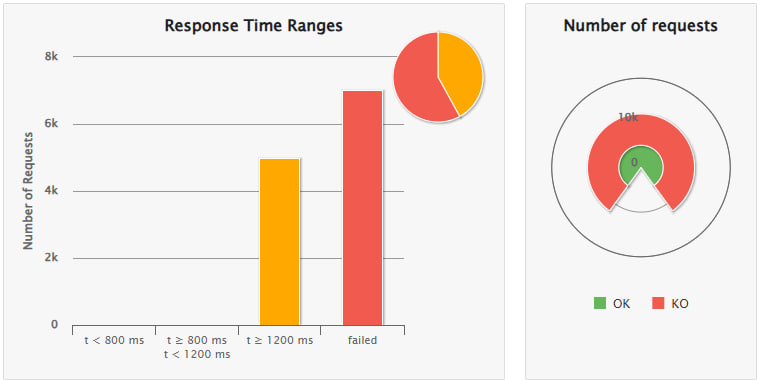
\includegraphics[width=0.8\linewidth]{images/sdk-gatling-high-graph.jpg}
    \caption{Raport wygenerowany w narzędziu Gatling dla aplikacji działającej w oparciu o podejście SDK, testowanej przy wysokim obciążeniu.}
    \label{fig:high}
    \vspace{0.5em}
    {\small Źródło: opracowanie własne.}
\end{figure}

\begin{itemize}
    \item Czas reakcji poniżej 800 ms: 0 żądań
    \item Czas reakcji od 800 ms do poniżej 1200 ms:  0 żądań
    \item Czas reakcji 1200 ms i więcej: Ponad 5000 żądań – dominująca część, silny wskaźnik przeciążenia systemu.
    \item Nieudane żądania: Około 7000 – aplikacja nie radzi sobie z obsługą dużej liczby żądań, występują błędy.
\end{itemize}

Porównanie wydajności:

\begin{itemize}
    \item Aplikacja działa optymalnie przy niskim obciążeniu — szybkie odpowiedzi, brak błędów i wysoka responsywność.
    \item Przy średnim obciążeniu wydajność ulega znacznemu pogorszeniu — dominują opóźnienia powyżej 1200 ms oraz wysoka liczba błędów.
    \item Wysokie obciążenie pokazuje dalsze pogorszenie — jeszcze więcej żądań ma bardzo długi czas odpowiedzi, a liczba nieudanych żądań sięga około 8000, co świadczy o przeciążeniu systemu.
\end{itemize}

\newpage

%biblioteki

Ocena współdzielenia kodu za pomocą bibliotek pod kątem skalowalności:

Biblioteki są zazwyczaj zoptymalizowane pod kątem konkretnego zadania w jednym języku. Jednak jeśli biblioteka nie jest zaprojektowana do pracy w środowiskach o dużej współbieżności, może wymagać dodatkowych zasobów sprzętowych w miarę wzrostu obciążenia. Na przykład intensywne przetwarzanie danych w bibliotekach może powodować większe zużycie pamięci lub CPU podczas pracy z dużymi zbiorami danych. Wspierająca myśl: Badania nad wydajnością obliczeniową często zauważają, że nieoptymalizowane biblioteki mogą stać się wąskimi gardłami pod dużym obciążeniem, prowadząc do zwiększenia kosztów zasobów fizycznych. ~\cite[p. 192]{fowler2012patterns}

W celu przygotowania analizy pod kątem skalowalności, tak samo jak w poprzednim przypadku opracowałem system, którego celem jest testowanie wydajności przykładowej aplikacji wykorzystującej biblioteki do współdzielenia kodu oraz obserwacja, w jaki sposób to podejście wpływa na wydajność i skalowalność systemu.

Przygotowane aplikacje przykładowe oraz kod systemu, który powstał w celu sprawdzenia i porównania wydajności, zostały dołączone do materiałów pracy.

Testowany system mikroserwisów składa się z dwóch mikroserwisów napisanych z użyciem technologii Java oraz Spring. Pierwszy mikroserwis produkuje dane, drugi je konsumuje. Oba serwisy uruchamiane są za pomocą narzędzia Docker. Kontenery Dockera mają ustawione limity zasobów, które mogą wykorzystywać.

Po uruchomieniu aplikacji w Dockerze, automatycznie uruchamiane są testy wydajnościowe przygotowane za pomocą narzędzia Gatling. Projekt został stworzony przy użyciu Javy, Springa oraz Gatlinga i znajduje się w materiałach dołączonych do pracy.

W trakcie testów wydajnościowych zbierane są metryki dotyczące użycia pamięci, liczby wątków, zużycia CPU, garbage collection i inne. Dane te są zapisywane do pliku za pomocą narzędzia Java Flight Recorder. Uruchomienie JFR odbywa się również automatycznie w momencie startu aplikacji.

Aplikacja testująca wydajność aplikacji przykładowej posiada trzy tryby testowania: małe obciążenie, średnie oraz duże. Zostało to zrealizowane w celu obserwacji działania aplikacji przy różnych poziomach obciążenia.

\newpage
% biblioteki meemery description

\begin{figure}
    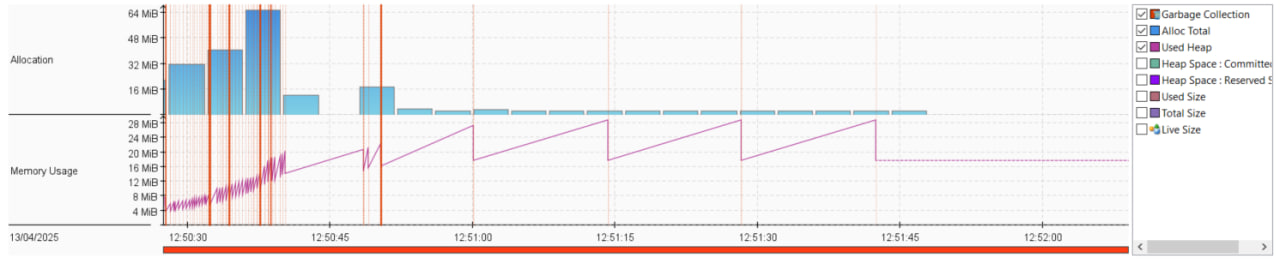
\includegraphics[width=\linewidth]{images/library-memory-low-graph.jpg}
    \caption{Wykres przedstawiający zużycie pamięci RAM aplikacji wykorzystującej biblioteki pod wpływem małego obciążenia.} \label{fig1}
    \vspace{0.5em}
    {\small Źródło: opracowanie własne.}
\end{figure}

Wyniki obserwacji:

Alokacja górny wykres — niebieskie słupki

\begin{itemize}
  \item Szczyty alokacji występują okresowo i zwykle nie przekraczają wartości 32~MiB.
  \item Widoczne są dłuższe przerwy pomiędzy zdarzeniami alokacji, co sugeruje rzadsze tworzenie obiektów i mniejsze zapotrzebowanie na pamięć.
  \item Po początkowej fazie obciążenia alokacja szybko stabilizuje się na niskim poziomie.
\end{itemize}

Garbage Collection – pionowe pomarańczowe linie

\begin{itemize}
  \item Liczba zdarzeń GC (Garbage Collection) jest stosunkowo niewielka.
  \item Mechanizm odśmiecania uruchamiany jest sporadycznie, co wynika z niskiego poziomu zużycia pamięci.
\end{itemize}

Wykorzystanie pamięci, dolny wykres – fioletowa linia

\begin{itemize}
  \item Wzrost zużycia sterty jest powolny i przewidywalny, osiągając maksymalnie około 24~MiB.
  \item Charakterystyczny jest łagodny wzrost z regularnymi, niewielkimi spadkami, które odpowiadają działaniu GC — co świadczy o stabilnym zarządzaniu pamięcią.
\end{itemize}

\newpage

\begin{figure}
    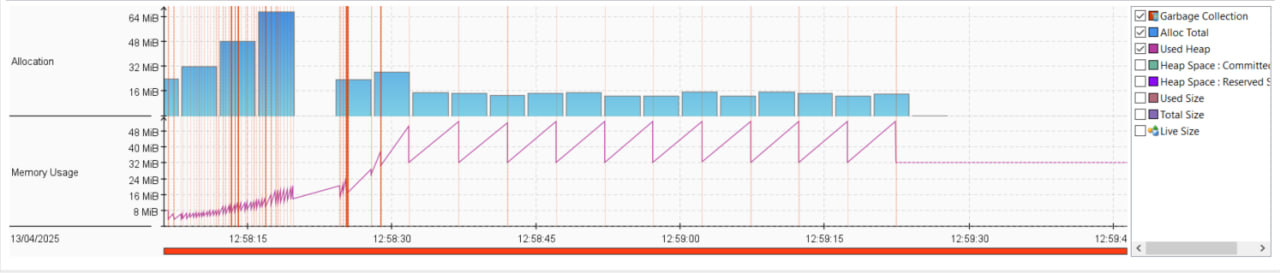
\includegraphics[width=\linewidth]{images/library-memory-midle-graph.jpg}
    \caption{Wykres przedstawiający zużycie pamięci RAM aplikacji wykorzystującej biblioteki pod wpływem średniego obciążenia.} \label{fig1}
    \vspace{0.5em}
    {\small Źródło: opracowanie własne.}
\end{figure}

W przypadku dużego obciążenia nie było możliwe wygenerowanie raportu ze względu na Memory Error.

Alokacja górny wykres — niebieskie słupki

\begin{itemize}
  \item Alokacja jest wyraźnie intensywniejsza i bardziej regularna.
  \item Maksymalne wartości alokacji dochodzą do 48~MiB, co wskazuje na wzmożone tworzenie obiektów w wyniku większej liczby żądań.
  \item Alokacje są utrzymywane przez dłuższy czas, a okresy bezczynności między kolejnymi słupkami są znacznie krótsze.
\end{itemize}

Garbage Collection – pionowe pomarańczowe linie

\begin{itemize}
  \item Zdarzenia GC są znacznie częstsze i bardziej cykliczne.
  \item Taki wzorzec odzwierciedla wzmożone wykorzystanie pamięci — więcej obiektów jest tworzonych i usuwanych, co jest typowe przy zwiększonym ruchu w aplikacji.
\end{itemize}

Wykorzystanie pamięci, dolny wykres – fioletowa linia

\begin{itemize}
  \item Użycie sterty wzrasta dynamiczniej i osiąga wartości nawet do 64~MiB.
  \item Fioletowa linia ukazuje klasyczny wzór zęba piły, który sugeruje intensywne cykle alokacji i czyszczenia pamięci.
  \item System zarządzania pamięcią reaguje odpowiednio na zwiększone obciążenie, ale wymaga częstszych interwencji GC.
\end{itemize}

<<<<<<< HEAD
Podsumowując, aplikacja w trakcie przeprowadzonych przeze mnie testów wykazała stabilne i efektywne zarządzanie pamięcią przy niskim i średnim obciążeniu. Jednak przy wysokim obciążeniu załamuje się, co może oznaczać ograniczenia w skalowalności.
=======
Podsumowując, aplikacja w rakcie przeprowadzonych trzeze mnie testów wykazała stabilne i efektywne zarządzanie pamięcią przy niskim i średnim obciążeniu, jednak załamuje się przy wysokim obciążeniu, co może oznaczać ograniczenia skalowalności.
>>>>>>> 64966de36be71826c93c5c7934c9ca0fa456c72c

\newpage

Raporty wygenerowane przez narzędzie Gatling:

%biblioteki gatling description

\begin{figure}
    \centering
    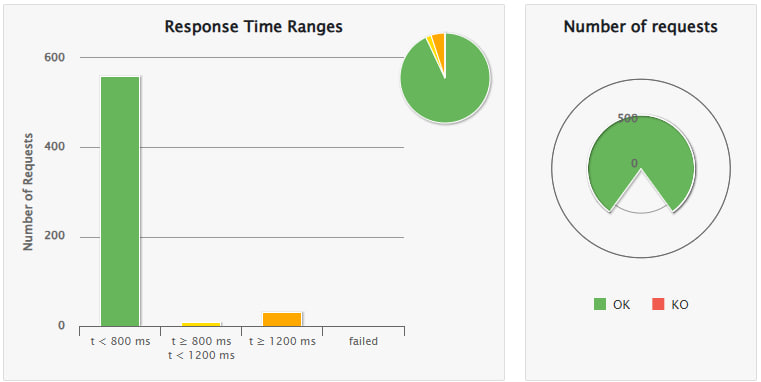
\includegraphics[width=0.8\linewidth]{images/library-gatling-low-graph.jpg}
    \caption{Raport wygenerowany w narzędziu Gatling dla aplikacji działającej w oparciu o biblioteki testowanej przy niskim obciążeniu.}
    \vspace{0.5em}
    {\small Źródło: opracowanie własne.}
    \label{fig:low}
\end{figure}

\begin{itemize}
    \item Czas reakcji poniżej 800 ms: Około 570 żądań – dobra wydajność, większość operacji wykonywana szybko.
    \item Czas reakcji od 800 ms do poniżej 1200 ms: Pojedyncze żądania – praktycznie brak wpływu na ogólną wydajność.
    \item Czas reakcji 1200 ms i więcej: Kilka żądań – sporadyczne opóźnienia, nieistotne z punktu widzenia użytkownika.
    \item Nieudane żądania: Brak – aplikacja działa niezawodnie.
\end{itemize}

\newpage

\begin{figure}
    \centering
    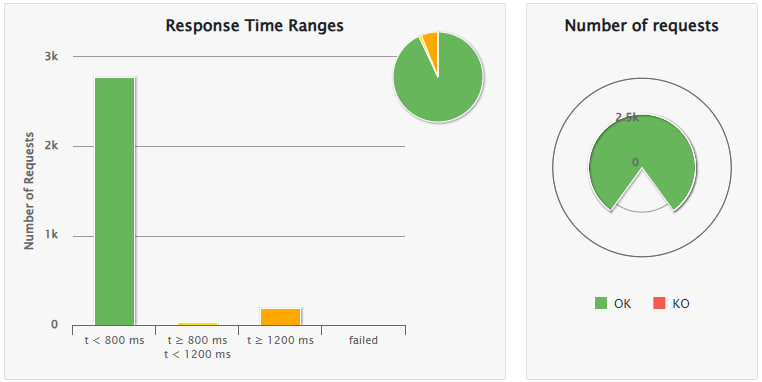
\includegraphics[width=0.8\linewidth]{images/library-gatling-middle-graph.jpg}
    \caption{Raport wygenerowany w narzędziu Gatling dla aplikacji działającej w oparciu o biblioteki testowanej przy średnim obciążeniu.}
    \vspace{0.5em}
    {\small Źródło: opracowanie własne.}
    \label{fig:middle}
\end{figure}

\begin{itemize}
    \item Czas reakcji poniżej 800 ms: Około 2700 żądań – wyraźna poprawa w porównaniu do testu średniego.
    \item Czas reakcji od 800 ms do poniżej 1200 ms: Około 10 żądań – minimalna liczba, pozytywny sygnał stabilizacji.
    \item Czas reakcji 1200 ms i więcej: Około 300 żądań – niewielkie opóźnienia nadal obecne, ale nie wpływają znacząco na ogólną ocenę.
    \item Nieudane żądania: Brak – aplikacja odzyskała stabilność i działa niezawodnie.
\end{itemize}

\newpage

\begin{figure}
    \centering
    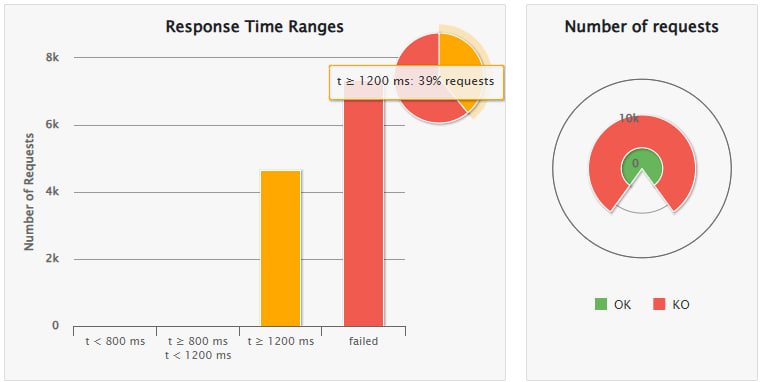
\includegraphics[width=0.8\linewidth]{images/library-gatling-high-graph.jpg}
    \caption{Raport wygenerowany w narzędziu Gatling dla aplikacji działającej w oparciu o biblioteki, testowanej przy wysokim obciążeniu.}
    \vspace{0.5em}
    {\small Źródło: opracowanie własne.}
    \label{fig:high}
\end{figure}

\begin{itemize}
    \item Czas reakcji poniżej 800 ms: Około 0 żądań – spadek w porównaniu do testu przy niskim obciążeniu.
    \item Czas reakcji od 800 ms do poniżej 1200 ms: Około 0 żądań – znaczny spadek, wskazujący na pogorszenie responsywności.
    \item Czas reakcji 1200 ms i więcej: Ponad 5000 żądań – dominująca część, silny wskaźnik przeciążenia systemu.
    \item Nieudane żądania: Około 7000 – aplikacja nie radzi sobie z obsługą dużej liczby żądań, występują błędy.
\end{itemize}

Wnioski dotyczące skalowalności:
\begin{itemize}
    \item Dobre zachowanie przy niskim i średnim obciążeniu
    \item Problemy ze skalowalnością przy wysokim obciążeniu
    \item Widoczna granica wydajności około 2500-3000 żądań
    \item Potrzeba optymalizacji zarządzania pamięcią przy dużym obciążeniu
\end{itemize}

<<<<<<< HEAD
Podsumowanie: Aplikacja wykorzystująca biblioteki wykazała w trakcie moich testów wysoką efektywność przy niskim i średnim obciążeniu. Jednak przy wysokim obciążeniu ujawnia problemy z zarządzaniem pamięcią.
=======
Podsumowanie: Aplikacja wykorzystująca biblioteki wykazła w trakcie mich testów wysoką efektywność przy niskim i średnim obciążeniu, jednak przy wysokim obciążeniu ujawnia problemy z zarządzaniem pamięcią.
>>>>>>> 64966de36be71826c93c5c7934c9ca0fa456c72c

\newpage

%rest

Ocena współdzielenia kodu za pomocą REST pod kątem skalowalności:

W celu przygotowania analizy pod kątem skalowalności, tak samo jak w poprzednim przypadku opracowałem system, którego celem jest testowanie wydajności przykładowej aplikacji wykorzystującej REST do współdzielenia kodu oraz obserwacja, w jaki sposób to podejście wpływa na wydajność i skalowalność systemu.

Przygotowane aplikacje przykładowe oraz kod systemu, który powstał w celu sprawdzenia i porównania wydajności, zostały dołączone do materiałów pracy.

Testowany system mikroserwisów składa się z dwóch mikroserwisów napisanych z użyciem technologii Java oraz Spring. Pierwszy mikroserwis produkuje dane, drugi je konsumuje. Oba serwisy uruchamiane są za pomocą narzędzia Docker. Kontenery Dockera mają ustawione limity zasobów, które mogą wykorzystywać.

Po uruchomieniu aplikacji w Dockerze, automatycznie uruchamiane są testy wydajnościowe przygotowane za pomocą narzędzia Gatling. Projekt został stworzony przy użyciu Javy, Springa oraz Gatlinga i znajduje się w materiałach dołączonych do pracy.

W trakcie testów wydajnościowych zbierane są metryki dotyczące użycia pamięci, liczby wątków, zużycia CPU, garbage collection i inne. Dane te są zapisywane do pliku za pomocą narzędzia Java Flight Recorder. Uruchomienie JFR odbywa się również automatycznie w momencie startu aplikacji.

Aplikacja testująca wydajność aplikacji przykładowej posiada trzy tryby testowania: małe obciążenie, średnie oraz duże. Zostało to zrealizowane w celu obserwacji działania aplikacji przy różnych poziomach obciążenia.

\newpage

%rest memory description

\begin{figure}
    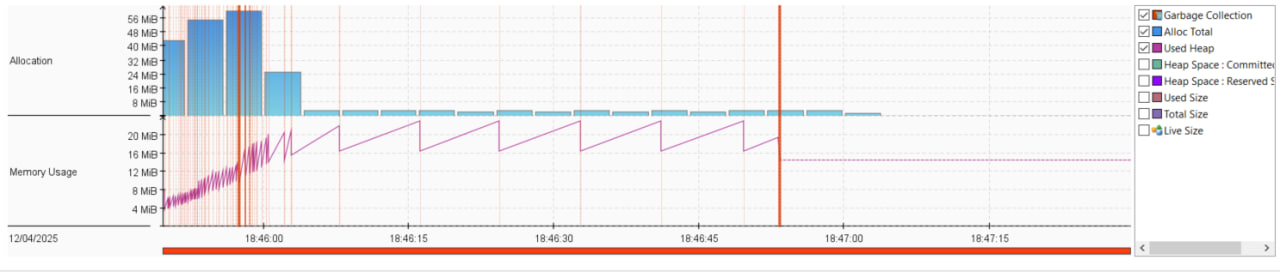
\includegraphics[width=\linewidth]{images/rest-memory-low-graph.jpg}
    \caption{Wykres przedstawiający zużycie pamięci RAM aplikacji wykorzystującej podejście REST pod wpływem małego obciążenia.} \label{fig1}
    \vspace{0.5em}
    {\small Źródło: opracowanie własne.}
\end{figure}

Wyniki obserwacji:

Alokacja górny wykres — niebieskie słupki

\begin{itemize}
  \item Szczyty alokacji są okresowe i zazwyczaj utrzymują się poniżej 32~MiB, co wskazuje na rzadkie tworzenie obiektów.
  \item Dłuższe okresy bezczynności pomiędzy zdarzeniami alokacji sugerują mniejszą liczbę żądań lub lżejsze przetwarzanie.
\end{itemize}

Garbage collection - pionowe pomarańczowe linie

\begin{itemize}
  \item Mniej zdarzeń GC, występujących sporadycznie z powodu niskiego obciążenia pamięci.
  \item Cykl GC prawdopodobnie prewencyjny, utrzymujący stabilną kondycję pamięci.
\end{itemize}

\newpage

\begin{figure}
    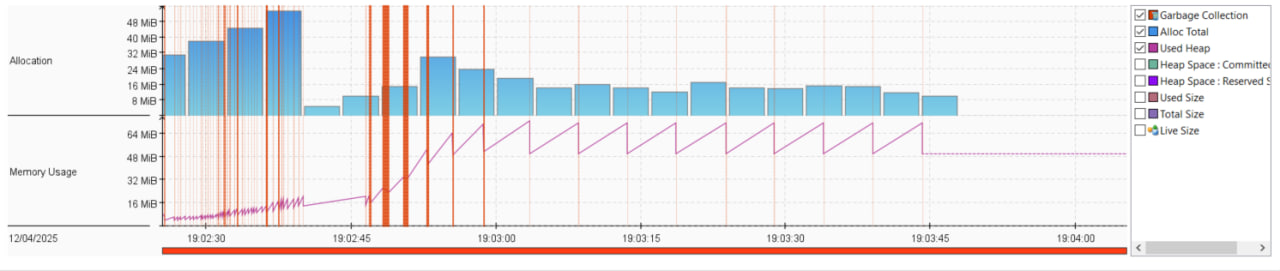
\includegraphics[width=\linewidth]{images/rest-memory-middle-graph.jpg}
    \caption{Wykres przedstawiający zużycie pamięci RAM aplikacji wykorzystującej podejście REST pod wpływem średniego obciążenia.} \label{fig1}
    \vspace{0.5em}
    {\small Źródło: opracowanie własne.}
\end{figure}

<<<<<<< HEAD
W przypadku dużego obciążenia wygenerowanie raportu nie było możliwe ze względu na błąd pamięci (Memory Error).
=======
W przypadku dużego obciążenia nie było możliwym wygenerowanie raportu ze względu na Memory Error.
>>>>>>> 64966de36be71826c93c5c7934c9ca0fa456c72c

Wyniki obserwacji:

Alokacja górny wykres — niebieskie słupki

\begin{itemize}
  \item Aktywność alokacji jest bardziej spójna, a szczyty sięgają 48~MiB.
  \item Krótsze przerwy między alokacjami wskazują na ciągłe tworzenie obiektów przy zwiększonej liczbie żądań.
  \item Brak najwyższego poziomu alokacji 64 MiB sugeruje umiarkowane, ale nie ekstremalne obciążenie.
\end{itemize}

\begin{itemize}
  \item Powolny, stabilny wzrost pamięci sterty do około 24~MiB, z niewielkimi spadkami po GC.
  \item Odzwierciedla przewidywalne zapotrzebowanie na pamięć i efektywne zarządzanie obiektami.
\end{itemize}

Garbage collection - pionowe pomarańczowe linie

\begin{itemize}
  \item Częstsze zdarzenia GC, skorelowane ze zwiększoną liczbą alokacji.
  \item Wskazuje na większą rotację obiektów tworzenie/niszczenie, choć nie tak intensywną jak przy wysokim obciążeniu.
\end{itemize}

Wykorzystanie pamięci dolny wykres — fioletowa linia

\begin{itemize}
  \item Szybszy wzrost do około 48~MiB, z regularnymi spadkami wynikającymi z agresywniejszych cykli GC.
  \item Wzorzec „wspinaczka i zrzut” wskazuje na cykliczne, ale kontrolowane zużycie pamięci.
\end{itemize}

\newpage

Raporty wygenerowane przez narzędzie Gatling:

%rest gatling description

\begin{figure}
    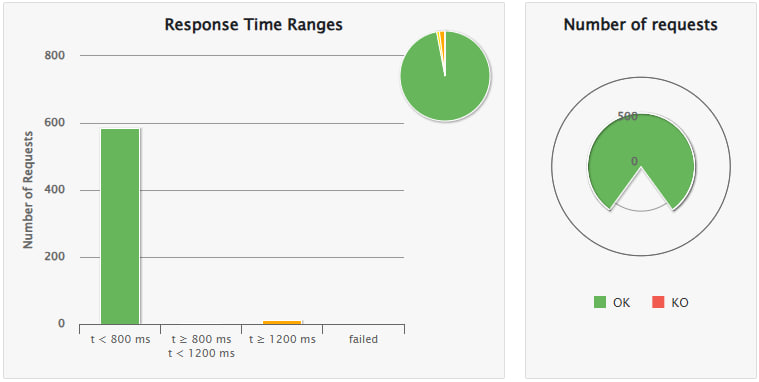
\includegraphics[width=\linewidth]{images/rest-gatling-low-graph.jpg}
    \caption{Raport wygenerowany w narzędziu Gatling dla aplikacji działającej w oparciu o podejście REST, testowanej przy niskim obciążeniu.} \label{fig1}
    \vspace{0.5em}
    {\small Źródło: opracowanie własne.}
\end{figure}

\begin{itemize}
  \item Analiza przy niskim obciążeniu:
  \begin{itemize}
    \item Dominujący czas odpowiedzi poniżej 800~ms (około 595 żądań)
    \item 0 żądań w przedziale 800-1200~ms
    \item Minimalna liczba żądań powyżej 1200~ms
    \item Brak żądań nieudanych (KO = 0)
  \end{itemize}
\end{itemize}

\newpage

\begin{figure}
    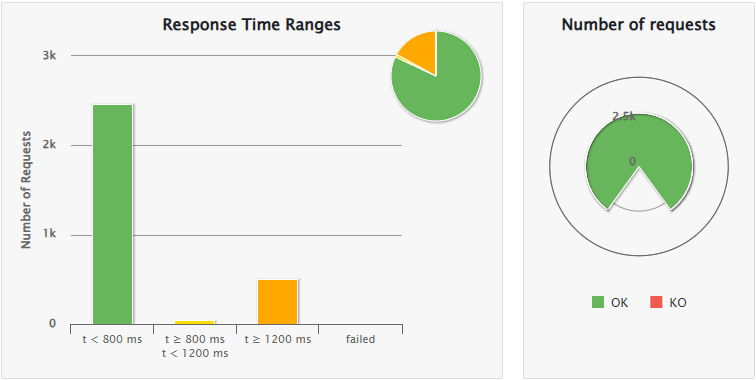
\includegraphics[width=\linewidth]{images/rest-gatling-middle-rest.jpg}
    \caption{Raport wygenerowany w narzędziu Gatling dla aplikacji działającej w oparciu o podejście REST, testowanej przy średnim obciążeniu.} \label{fig2}
    \vspace{0.5em}
    {\small Źródło: opracowanie własne.}
\end{figure}

\begin{itemize}
  \item Analiza przy średnim obciążeniu:
  \begin{itemize}
    \item Około 2400 żądań poniżej 800~ms - zauważalny spadek wydajności
    \item Mała liczba żądań w przedziale 800-1200~ms
    \item Pojawienie się około 500 żądań powyżej 1200~ms
    \item Minimalna liczba nieudanych żądań, system zachowuje stabilność
  \end{itemize}
\end{itemize}

\newpage

\begin{figure}
    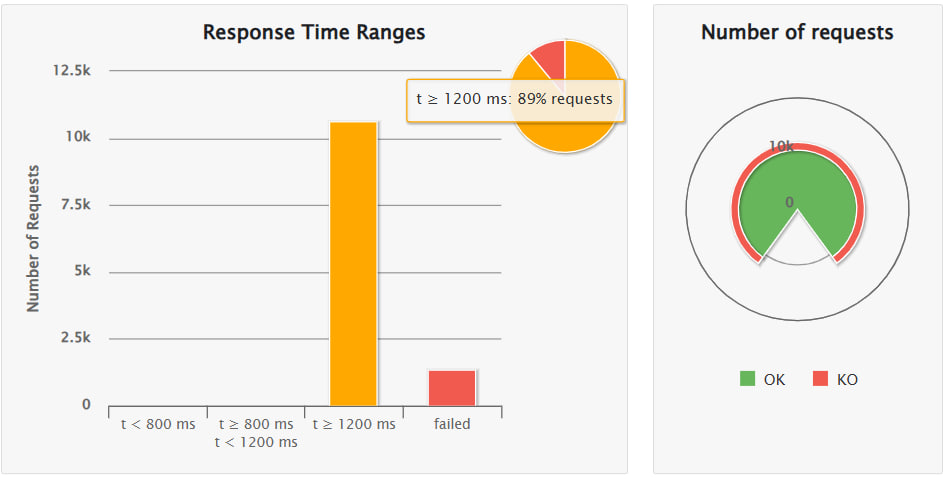
\includegraphics[width=\linewidth]{images/rest-gatling-high-graph.jpg}
    \caption{Raport wygenerowany w narzędziu Gatling dla aplikacji działającej w oparciu o podejście REST, testowanej przy wysokim obciążeniu.} \label{fig3}
    \vspace{0.5em}
    {\small Źródło: opracowanie własne.}
\end{figure}

\begin{itemize}
  \item Analiza przy wysokim obciążeniu:
  \begin{itemize}
    \item Brak odpowiedzi poniżej 800~ms
    \item 0 żądań w przedziale 800-1200~ms
    \item Około 89 procentów żądań (7500-10000) powyżej 1200~ms
    \item Znacząca liczba nieudanych żądań wskazująca na przeciążenie systemu
  \end{itemize}
\end{itemize}

<<<<<<< HEAD
Podsumowując, podejście REST w trakcie moich testów wykazało dobrą wydajność przy niskim obciążeniu, ale znacząco traci na efektywności wraz ze wzrostem liczby żądań. Przy wysokim obciążeniu system ujawnia poważne problemy z wydajnością — obserwuję długie czasy odpowiedzi oraz występowanie błędów.
=======
Podsumowując, podejście REST, w trakcie moich testów wykazało dobrą wydajność przy niskim obciążeniu, ale znacząco traci na efektywności wraz ze wzrostem liczby żądań. Przy wysokim obciążeniu system ujawnia poważne problemy z wydajnością, obserwuję długie czasy odpowiedzi i występowanie błędów.
>>>>>>> 64966de36be71826c93c5c7934c9ca0fa456c72c

\newpage

% descripion here

%severless

Ocena współdzielenia kodu za pomocą Serverless pod kątem skalowalności:

W celu przygotowania analizy pod kątem skalowalności, tak samo jak w poprzednim przypadku opracowałem system, którego celem jest testowanie wydajności przykładowej aplikacji wykorzystującej Serverless do współdzielenia kodu oraz obserwacja, w jaki sposób to podejście wpływa na wydajność i skalowalność systemu.

Przygotowane aplikacje przykładowe oraz kod systemu, który powstał w celu sprawdzenia i porównania wydajności, zostały dołączone do materiałów pracy.

Testowany system mikroserwisów składa się z dwóch mikroserwisów napisanych z użyciem technologii Java oraz Spring. Pierwszy mikroserwis produkuje dane, drugi je konsumuje. Oba serwisy uruchamiane są za pomocą narzędzia Docker. Kontenery Dockera mają ustawione limity zasobów, które mogą wykorzystywać.

Po uruchomieniu aplikacji w Dockerze, automatycznie uruchamiane są testy wydajnościowe przygotowane za pomocą narzędzia Gatling. Projekt został stworzony przy użyciu Javy, Springa oraz Gatlinga i znajduje się w materiałach dołączonych do pracy.

W trakcie testów wydajnościowych zbierane są metryki dotyczące użycia pamięci, liczby wątków, zużycia CPU, garbage collection i inne. Dane te są zapisywane do pliku za pomocą narzędzia Java Flight Recorder. Uruchomienie JFR odbywa się również automatycznie w momencie startu aplikacji.

<<<<<<< HEAD
Aplikacja testująca wydajność aplikacji przykładowej oferuje trzy tryby testowania: małe, średnie oraz duże obciążenie. Zostało to wdrożone w celu obserwacji działania aplikacji przy różnych poziomach obciążenia.
=======
Aplikacja testująca wydajność aplikacji przykładowej posiada trzy tryby testowania: małe obciążenie, średnie oraz duże. Zostało to zrealizowane w celu obserwacji działania aplikacji pod wpływem różnych poziomów obciążenia.
>>>>>>> 64966de36be71826c93c5c7934c9ca0fa456c72c

\newpage
%serverless memory description

\begin{figure}
    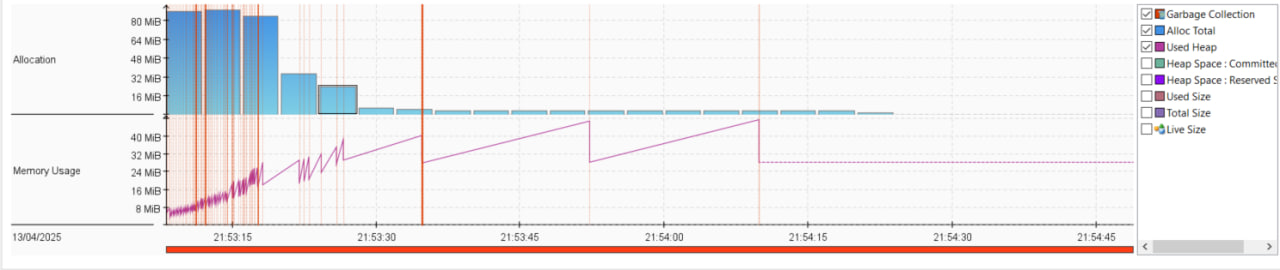
\includegraphics[width=\linewidth]{images/serverless-memory-low-graph.jpg}
    \caption{Wykres przedstawiający zużycie pamięci RAM aplikacji wykorzystującej podejście Serverless pod wpływem małego obciążenia.} \label{fig1}
    \vspace{0.5em}
    {\small Źródło: opracowanie własne.}
\end{figure}

Wyniki obserwacji:

Alokacja pamięci (niebieskie słupki)

\begin{itemize}
    \item Szczyty alokacji są bardzo niskie, utrzymujące się w okolicach 9~MB.
    \item Brak wyraźnych okresowych wzorców, co sugeruje sporadyczne i minimalne tworzenie obiektów.
    \item Wykres wskazuje na bardzo małe obciążenie systemu, z rzadkimi zdarzeniami alokacji.
\end{itemize}

Zbieranie śmieci (pionowe pomarańczowe linie)

\begin{itemize}
    \item Bardzo rzadkie zdarzenia GC, co jest spodziewane przy minimalnym wykorzystaniu pamięci.
    \item Brak wyraźnych sygnałów GC na wykresie, co potwierdza niską aktywność systemu.
\end{itemize}

Wykorzystanie pamięci (linie fioletowe)

\begin{itemize}
    \item Wykorzystanie pamięci jest stabilne i bardzo niskie, oscylujące wokół 9~MB.
    \item Brak znaczących wahań, co wskazuje na brak presji na pamięć.
\end{itemize}

\newpage

\begin{figure}
    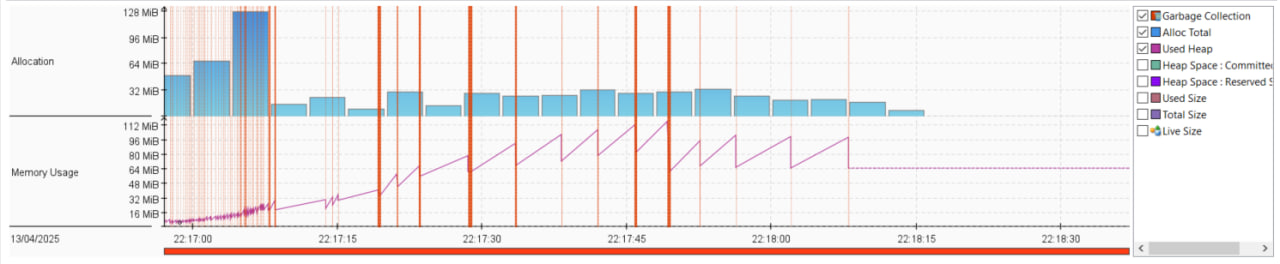
\includegraphics[width=\linewidth]{images/serverless-memory-middle-graph.jpg}
    \caption{Wykres przedstawiający zużycie pamięci RAM aplikacji wykorzystującej podejście Serverless pod wpływem średniego obciążenia.} \label{fig1}
    \vspace{0.5em}
    {\small Źródło: opracowanie własne.}
\end{figure}

W przypadku dużego obciążenia nie było możliwe wygenerowanie raportu ze względu na Memory Error.

<<<<<<< HEAD
Wyniki mojej obserwacji
=======
Wyniki mojej obserwacji:
>>>>>>> 64966de36be71826c93c5c7934c9ca0fa456c72c

Alokacja pamięci (niebieskie słupki)

\begin{itemize}
    \item Aktywność alokacji jest znacznie wyższa, z wartościami sięgającymi 12~MB.
    \item Występuje bardziej regularny wzorzec alokacji, wskazujący na ciągłe przetwarzanie żądań.
    \item Zwiększona częstotliwość alokacji sugeruje większe obciążenie systemu w porównaniu do scenariusza niskiego obciążenia.
\end{itemize}

Zbieranie śmieci (pionowe pomarańczowe linie)

\begin{itemize}
    \item Częstsze zdarzenia GC, choć nie są one bardzo intensywne.
    \item Występowanie GC jest związane ze zwiększoną alokacją obiektów, ale nie osiąga poziomu agresywnego czyszczenia.
\end{itemize}

Wykorzystanie pamięci (linie fioletowe)

\begin{itemize}
    \item Wykorzystanie pamięci jest wyższe, osiągając wartości do 128~MB, ale z częstymi spadkami.
    \item Wykres pokazuje okresowe wzrosty i spadki, co sugeruje cykle alokacji i zwalniania pamięci.
    \item System radzi sobie z obciążeniem, ale wymaga częstszego odśmiecania.
\end{itemize}

% Dodatkowe obserwacje:
% \begin{itemize}
%     \item Niskie obciążenie: System działa w stanie bliskim bezczynności, z minimalnym wykorzystaniem zasobów. Idealny dla prostych zadań o niskiej częstotliwości.
%     \item Średnie obciążenie: System jest bardziej aktywny, ale wciąż efektywnie zarządza pamięcią. Wykresy wskazują na dobrą równowagę między alokacją a GC.
%     \item W obu przypadkach brak oznak przecieku pamięci, ale średnie obciążenie wymaga bliższego monitorowania pod kątem wydajności.
% \end{itemize}

\newpage

%serverless gatling description

Raporty wygenerowane przez narzędzie Gatling:

\begin{figure}
    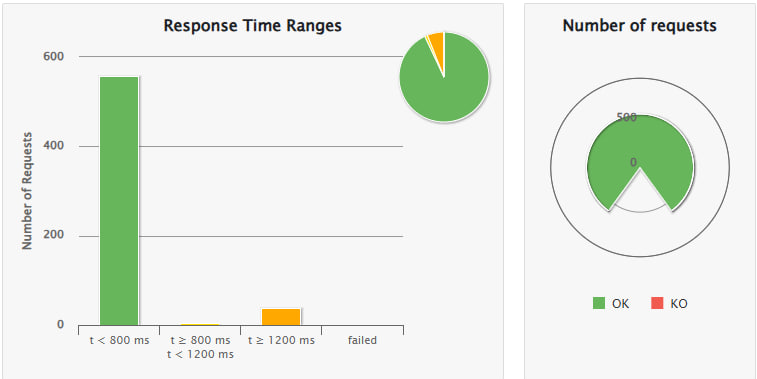
\includegraphics[width=\linewidth]{images/serverless-gatling-low-graph.jpg}
    \caption{Raport wygenerowany w narzędziu Gatling dla aplikacji działającej w oparciu o podejście Serverless, testowanej przy niskim obciążeniu.} \label{fig1}
    \vspace{0.5em}
    {\small Źródło: opracowanie własne.}
\end{figure}

\begin{itemize}
  \item Analiza przy niskim obciążeniu:
  \begin{itemize}
    \item Dominująca liczba żądań (580) z czasem odpowiedzi poniżej 800~ms
    \item Minimalna liczba żądań w przedziale 800-1200~ms
    \item Mała liczba żądań powyżej 1200~ms
    \item Brak żądań nieudanych - pełna niezawodność
  \end{itemize}
\end{itemize}

\newpage

\begin{figure}
    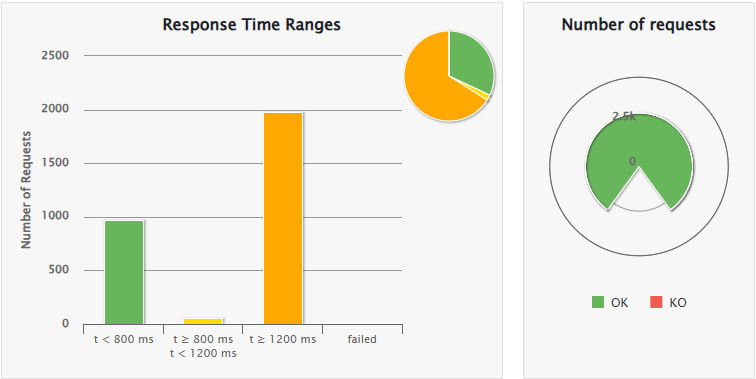
\includegraphics[width=\linewidth]{images/serverless-gatling-middle-graph.jpg}
    \caption{Raport wygenerowany w narzędziu Gatling dla aplikacji działającej w oparciu o podejście Serverless, testowanej przy średnim obciążeniu.} \label{fig2}
    \vspace{0.5em}
    {\small Źródło: opracowanie własne.}
\end{figure}

\begin{itemize}
  \item Analiza przy średnim obciążeniu:
  \begin{itemize}
    \item Około 1000 żądań poniżej 800~ms - poprawa względem poprzedniego testu
    \item Minimalna liczba żądań w przedziale 800-1200~ms
    \item 2000 żądań powyżej 1200~ms
    \item Utrzymana pełna niezawodność - brak żądań nieudanych
  \end{itemize}
\end{itemize}

\newpage

\begin{figure}
    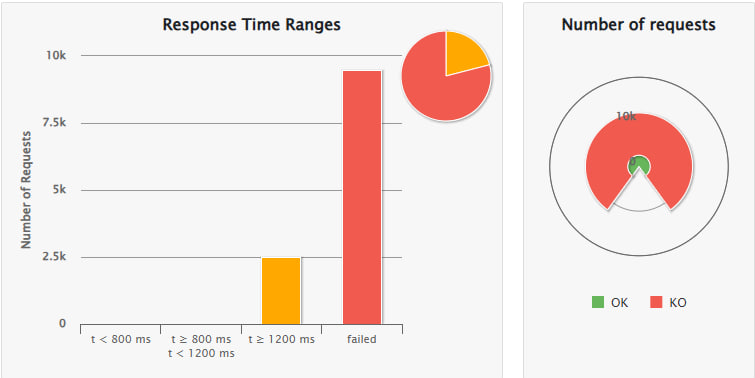
\includegraphics[width=\linewidth]{images/serverless-gatling-high-graph.jpg}
    \caption{Raport wygenerowany w narzędziu Gatling dla aplikacji działającej w oparciu o podejście Serverless, testowanej przy wysokim obciążeniu.} \label{fig3}
    \vspace{0.5em}
    {\small Źródło: opracowanie własne.}
\end{figure}

\begin{itemize}
  \item Analiza przy wysokim obciążeniu:
  \begin{itemize}
    \item 0 żądań poniżej 800~ms
    \item 0 żądań w przedziale 800-1200~ms
    \item 39 procentów żądań powyżej 1200~ms
    \item Bardzo duża liczba żądań nieudanych
  \end{itemize}
\end{itemize}

\begin{itemize}
  \item Podsumowanie wyników:
  \begin{itemize}
    \item Niskie obciążenie: Optymalna wydajność z szybkim czasem reakcji
    \item Średnie obciążenie: Stabilna wydajność z niewielkimi opóźnieniami
    \item Wysokie obciążenie: Znaczące pogorszenie wydajności i stabilności
  \end{itemize}
\end{itemize}

<<<<<<< HEAD
Możemy zaobserwować pogorszenie wydajności, szczególnie przy większych obciążeniach. Prawdopodobnie wynika to z opóźnień sieciowych spowodowanych przez architekturę serverless.
=======
Możeny zaobserwować pogorszenie wydajności, szczególnie przy większych obciążeniach, prawdopodobnie wynika to z opóźnienia sieciowego spowodowanego przez architekturę serverless.
>>>>>>> 64966de36be71826c93c5c7934c9ca0fa456c72c

\newpage

%wyniki analizy wydajnościowej

%AI
Podsumowanie wyników testowania rozwiązań pod kątem wydajności i skalowalności.

<<<<<<< HEAD
Przygotowałem ranking rozwiązań pod względem wydajności i skalowalności, oparty na przeprowadzonych testach i analizach:
=======
Przygotowałem ranking rozwiązań pod względem wydajności i skalowalności, który stworzyłem na podstawie przeprowadzonych testów i analiz:
>>>>>>> 64966de36be71826c93c5c7934c9ca0fa456c72c

\begin{enumerate}
    \item Serverless
    \begin{itemize}
        \item Wydajność:
        \begin{itemize}
            \item Bardzo wydajne wykorzystanie pamięci (9MB przy niskim obciążeniu)
            \item Spójna wydajność z większością żądań poniżej 800ms
        \end{itemize}
        \item Skalowalność:
        \begin{itemize}
            \item Automatyczne skalowanie w zależności od obciążenia
            \item Efektywne zarządzanie zasobami przy zmiennym obciążeniu
            \item Najlepsza elastyczność przy nagłych skokach ruchu
        \end{itemize}
    \end{itemize}

    \item IDL (Interface Definition Language)
    \begin{itemize}
        \item Wydajność:
        \begin{itemize}
            \item Najlepsza gospodarka pamięcią (szczyty około 32 MiB)
            \item Najbardziej spójne czasy odpowiedzi poniżej 800ms
            \item Doskonałe wzorce garbage collection
        \end{itemize}
        \item Skalowalność:
        \begin{itemize}
            \item Dobra skalowalność horyzontalna
            \item Wymaga ręcznej konfiguracji skalowania
            \item Stabilna wydajność przy zwiększającym się obciążeniu
        \end{itemize}
    \end{itemize}

    \item Biblioteki
    \begin{itemize}
        \item Wydajność:
        \begin{itemize}
            \item Umiarkowane wykorzystanie pamięci (150-200MB)
            \item Dobra wydajność przy niskim obciążeniu
        \end{itemize}
        \item Skalowalność:
        \begin{itemize}
            \item Ograniczona skalowalność automatyczna
            \item Wymaga dodatkowej infrastruktury do skalowania
            \item Stabilna przy przewidywalnym obciążeniu
        \end{itemize}
    \end{itemize}

    \item SDK
    \begin{itemize}
        \item Wydajność:
        \begin{itemize}
            \item Wyższe zużycie pamięci
            \item Częstsze zdarzenia garbage collection
        \end{itemize}
        \item Skalowalność:
        \begin{itemize}
            \item Trudniejsza w implementacji skalowalność
            \item Wyższe koszty skalowania
            \item Znacząca degradacja przy wysokim obciążeniu
        \end{itemize}
    \end{itemize}

    \item REST
    \begin{itemize}
        \item Wydajność:
        \begin{itemize}
            \item Najwyższe zużycie pamięci
            \item Najwyższy procent powolnych odpowiedzi (>1200ms)
        \end{itemize}
        \item Skalowalność:
        \begin{itemize}
            \item Najbardziej problematyczna skalowalność
            \item Wysokie ryzyko błędów przy skalowaniu
            \item Znaczące koszty infrastruktury przy skalowaniu
        \end{itemize}
    \end{itemize}
\end{enumerate}

Wnioski końcowe

<<<<<<< HEAD
Na podstawie przeprowadzonej analizy mogę stwierdzić, że wybór optymalnego rozwiązania zależy od specyficznych wymagań projektu. Jednak, biorąc pod uwagę zarówno wydajność, jak i skalowalność, architektura Serverless oraz IDL wykazują najlepsze właściwości.
=======
Na podstawie przeprowadzonej analizy mogę stwierdzić, że wybór optymalnego rozwiązania zależy od specyficznych wymagań projektu, jednak biorąc pod uwagę zarówno wydajność, jak i skalowalność, architektura Serverless oraz IDL wykazują najlepsze właściwości.
>>>>>>> 64966de36be71826c93c5c7934c9ca0fa456c72c

Serverless zajmuje pierwsze miejsce głównie ze względu na:
\begin{itemize}
    \item Automatyczną skalowalność bez potrzeby ręcznej konfiguracji
    \item Najniższe zużycie zasobów przy zmiennym obciążeniu
    \item Optymalne zarządzanie kosztami w zależności od rzeczywistego wykorzystania
\end{itemize}

IDL plasuje się na drugim miejscu, oferując:
\begin{itemize}
    \item Najlepszą wydajność przy stałym obciążeniu
    \item Przewidywalną skalowalność
    \item Niższe koszty operacyjne przy stałym, wysokim obciążeniu
\end{itemize}

<<<<<<< HEAD
Uważam, że biblioteki stanowią rozsądny kompromis dla projektów o średnich rozmiarach, podczas gdy SDK i REST wykazują największe trudności w kontekście skalowalności i wydajności przy większym obciążeniu.

Moje rekomendacje, przygotowane na podstawie przeprowadzonego badania:
=======
Uważam że biblioteki stanowią rozsądny kompromis dla projektów o średnich rozmiarach, podczas gdy SDK i REST wykazują największe trudności w kontekście skalowalności i wydajności przy większym obciążeniu.

Moje rekomendacje przygotowane na podstawie przeprowadzonego badania:
>>>>>>> 64966de36be71826c93c5c7934c9ca0fa456c72c

\begin{itemize}
    \item Dla projektów z dynamicznym obciążeniem: Serverless
    \item Dla projektów ze stałym, wysokim obciążeniem: IDL
    \item Dla projektów średniej wielkości z przewidywalnym obciążeniem: Biblioteki
    \item Unikać REST i SDK w przypadku wymagań dotyczących wysokiej skalowalności
\end{itemize}

<<<<<<< HEAD
Uważam, że musimy wziąć pod uwagę fakt, że w każdym z przeprowadzonych przeze mnie testów z wysokim obciążeniem występowały błędy związane z pamięcią RAM, z czego mogę wyciągnąć wniosek, że niezbędne jest planowanie pojemności oraz implementacja strategii skalowania, niezależnie od wybranego rozwiązania lub podejścia do współdzielenia kodu.
=======
%100AI
Uwarzam że musimy wiciąć pod uwagę to, że w każdym z przeprowadzonych przeze mnie testów z wysokim ociążeniem występowały błędy związanie z pamięcią RAM, z czego mogę wyciągnąć wniosek, że niezbędnym jest  planowania pojemności i implementacji strategii skalowania, niezależnie od wybranego rozwiązania lub podejścia do współdzielenia kodu.
%Należy jednak pamiętać, że błędy pamięci przy wysokim obciążeniu były obecne we wszystkich podejściach, co podkreśla znaczenie właściwego planowania pojemności i implementacji strategii skalowania, niezależnie od wybranego rozwiązania.
>>>>>>> 64966de36be71826c93c5c7934c9ca0fa456c72c
%end wyniki analizy wydajności

% scalability end

\section{Opis części praktycznej}

%100AI

Jako część praktyczną mojej pracy magisterskiej przygotowałem aplikację webową, która składa się z dwóch części, backendowej i frontendowej.
Głównym celem napisania aplikacji jest wprowadzenie nowego podejścia do współdzielenia kodu – współdzielenie za pomocą technologii serverless. Aplikacja wspiera deweloperów korzystających z technologii serverless, zmniejsza wady tego rozwiązania, jednocześnie dając możliwość skorzystania z mocnych stron tej technologii.

Czym jest technologia Serverless?

<<<<<<< HEAD
Serverless to nowoczesny model wykonywania obliczeń, w którym dostawcy chmury automatycznie obsługują aspekty infrastruktury, takie jak zarządzanie fizycznymi serwerami oraz skalowanie zasobów przydzielonych każdemu klientowi. Zamiast zarządzać serwerami fizycznymi lub wirtualnymi, programiści mogą skupić się wyłącznie na pisaniu kodu. Termin „serverless” nie oznacza braku fizycznych serwerów, lecz to, że zarządzaniem nimi zajmuje się dostawca usług chmurowych. W architekturze serverless do chmury przesyła się pojedyncze funkcje zamiast całych aplikacji, a dostawca chmury odpowiada za zarządzanie kodem, skalowanie i utrzymanie tych funkcji. Są one często nazywane Function-as-a-Service (FaaS).
=======
%100AI

Serverless to nowoczesny model wykonywania obliczeń, w którym dostawcy chmury automatycznie obsługują aspekty infrastruktury, takie jak zarządzanie fizycznym serwerem, skalowanie zasobów przydzielonych każdemu klientowi. Zamiast zarządzania serwerami fizycznymi lub wirtualnymi, programiści mogą skupić się wyłącznie na pisaniu kodu. Termin „serverless” nie oznacza, że nie ma fizycznych serwerów, ale że zarządzaniem serwerem zajmuje się dostawca usług chmurowych. W architekturze serverless możemy do chmury pojedyncze funkcje zamiast całych aplikacji, a dostawca chmury jest odpowiedzialny za zarządzanie kodem, skalowanie i utrzymywanie tych funkcji. Są one też często nazywane Function-as-a-Service (FaaS).
>>>>>>> 64966de36be71826c93c5c7934c9ca0fa456c72c

Przykłady platform Serverless dostępnych w 2025 roku:

\begin{enumerate}
    \item AWS Lambda
    \item Azure Functions
    \item Google Cloud Functions
    \item IBM Cloud Functions
\end{enumerate}

\subsubsection{Ogólny opis aplikacji}

Przygotowana aplikacja webowa realizuje następujące funkcje:

\begin{enumerate}
    \item Akceptacja i sprawdzanie kodu, który użytkownik chce podzielić za pomocą technologii serverless. W przypadku problemów podczas sprawdzania, aplikacja informuje użytkownika, co należy zrobić, aby zakończyć proces pomyślnie.
    \item Automatyczne przygotowanie kodu do wdrożenia na Amazon Lambda (w przyszłości możliwe będzie dodanie opcji wyboru innej platformy, np. Azure Functions).
    \item Automatyczne wdrażanie kodu na platformę Serverless, który po chwili staje się dostępny.
    \item Zapisywanie kodu w bazie danych, umożliwiając jego późniejsze wykorzystanie; użytkownik ma dostęp do listy wszystkich wdrożonych fragmentów kodu.
    \item Możliwość edytowania i ponownego wdrażania kodu z listy.
    \item Możliwość wyszukiwania kodu po opisie.
    \item Obsługa wersjonowania kodu.
    \item Automatyczne przygotowywanie plików IDL, które są przydatne do wykorzystania, gdy kod jest wywoływany przez IDL.
    \item Przechowywanie plików IDL, które użytkownik może udostępnić innym członkom zespołu w celu współdzielenia kodu.
\end{enumerate}

\subsubsection{Opis aplikacji back-end}

Używane technologie

\begin{enumerate}
    \item Java - Język programowania wykorzystany do implementacji części serwerowej aplikacji.
    \item Spring Boot - Framework ułatwiający tworzenie aplikacji w języku Java, oferujący gotowe rozwiązania dla typowych problemów programistycznych.
    \item Maven - Narzędzie automatyzujące proces budowania aplikacji, zarządzania zależnościami oraz kompilacji projektów.
    \item AWS Lambda - Usługa obliczeniowa typu serverless, która umożliwia uruchamianie kodu bez konieczności zarządzania serwerami, gdzie dostawca chmury odpowiada za infrastrukturę.
    \item Protobuf - Język IDL służący do szybkiego kodowania i dekodowania obiektów DTO.
    \item Jackson - Biblioteka do parsowania danych w formacie JSON oraz konwertowania ich na obiekty DTO i odwrotnie.
\end{enumerate}

Ogólny opis

Ta aplikacja jest częścią aplikacji webowej, która odpowiada za następujące działania:
\begin{enumerate}
    \item Odbiera kod jako dane wejściowe użytkownika - Akceptuje kod od użytkownika za pośrednictwem żądań HTTP.
    \item Weryfikuje kod - Sprawdza, że otrzymany kod spełnia wymagane standardy i format.
    \item Automatycznie wdraża kod jako funkcję Lambda -  Wdraża sprawdzony kod jako funkcję AWS Lambda.
    \item Generuje pliki .proto - Tworzy pliki .proto na podstawie kodu wejściowego, które mogą być używane do generowania obiektów DTO do komunikacji z wdrożoną funkcją Lambda.
\end{enumerate}


\subsubsection{Opis aplikacji front-end}

Aplikację front-endową przygotowałem za pomocą JavaScript, React i npm.
React to biblioteka używana do tworzenia aplikacji frontendowych, a npm służy do zarządzania zależnościami projektu.

Ogólny opis:

Ta aplikacja jest częścią aplikacji webowej. Część front-endowa jest odpowiedzialna za następujące działania:
\begin{enumerate}
    \item Przyjmowanie kodu, który użytkownik chce współdzielić, a następnie wysyłanie go do serwera back-endowego.
    \item Weryfikacja tego, czy kod spełnia wymagane standardy i formatowanie.
    \item Wyświetlanie wyników walidacji.
    \item Możliwość przeglądania, edytowania i usuwania kodu, który został wcześniej zapisany i wdrożony w AWS Lambda.
    \item Możliwość wyszukiwania wdrożonego kodu, używając jego opisu i nazwy.
    \item Wsparcie wersjonowania kodu w celu śledzenia zmian lub przywracania poprzednich wersji.
    \item Udostępnianie plików .proto: aplikacja front-end udostępnia użytkownikom wygenerowane pliki .proto, których użytkownicy mogą użyć do generowania obiektów DTO dla komunikacji z wdrożoną funkcją Lambda.
\end{enumerate}

\newpage

\begin{figure}[H] % [H] forces the figure to stay HERE using the float package
    \centering
    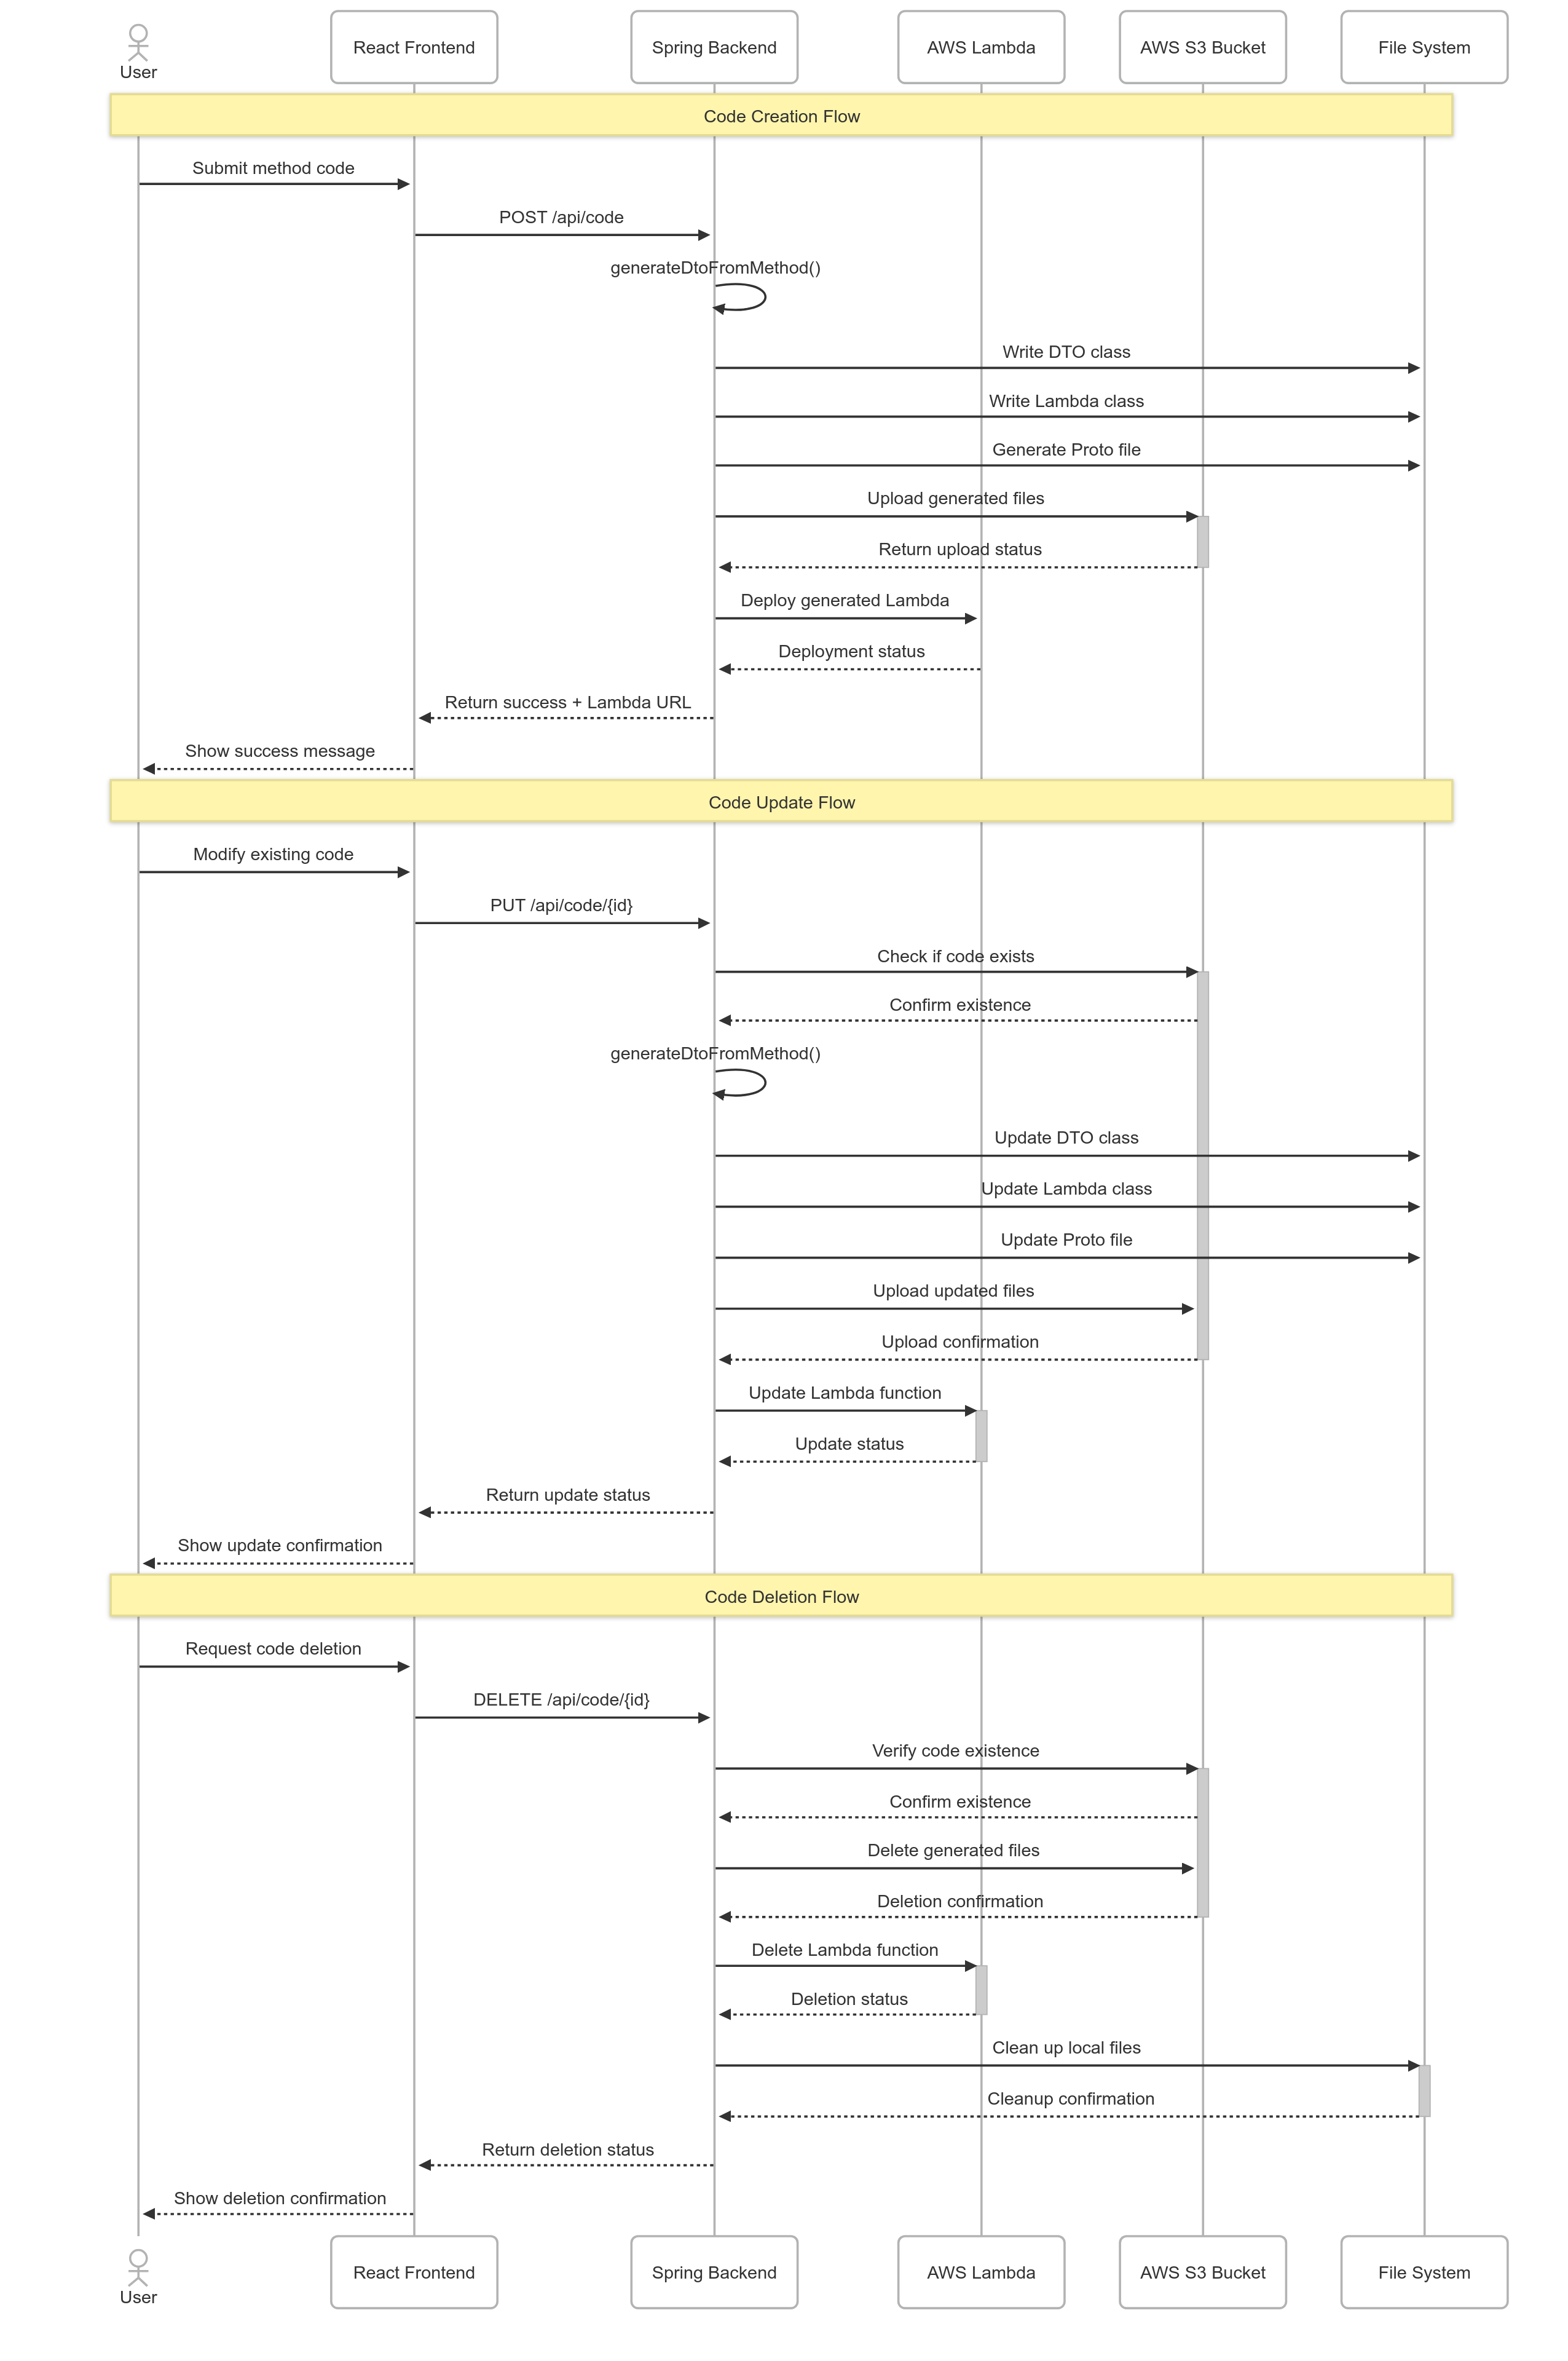
\includegraphics[width=\linewidth]{images/sequentinal-diagram.png}
    \caption{Diagram sekwencyjny działania aplikacji praktycznej}
    \label{fig2}
    \vspace{0.5em}
    {\small Źródło: opracowanie własne.}
\end{figure}

\newpage

%start of code report

\subsection{Przedstawienie ważnych fragmentów kodu}

Chcę przedstawić kluczowe fragmenty kodu mojego projektu praktycznego wraz z krótkim opisem ich działania.

Poniżej przedstawiono podstawową konfigurację usługi Lambda przy użyciu klienta AWS.

Klasa inicjalizuje klientów usług AWS. W moim przypadku są to: S3Client, LambdaClient oraz IamClient, które służą odpowiednio do zarządzania funkcjami Lambda, przechowywania danych w S3 oraz zarządzania rolami IAM.

\begin{verbatim}
@Service
public class LambdaService {
    private final String bucketName = "lambda-jars";
    private final String roleName = "lambda-execution-role";
    private final String jarFilePath = "path/to/jar";

    private final S3Client s3Client;
    private final LambdaClient lambdaClient;
    private final IamClient iamClient;

    public LambdaService(S3Client s3Client, LambdaClient lambdaClient,
                        IamClient iamClient) {
        this.s3Client = s3Client;
        this.lambdaClient = lambdaClient;
        this.iamClient = iamClient;
    }
}
\end{verbatim}

Poniższy kod wykonuje budowanie pliku JAR za pomocą Mavena, a następnie przesyła go do S3 oraz tworzy nową funkcję Lambda z odpowiednią rolą IAM.

\begin{verbatim}
public void prepareJarForLambda(String id) {
    System.setProperty("maven.multiModuleProjectDirectory", "path/to/project");
    System.setProperty("maven.home", "path/to/maven");
    System.setProperty("JAVA_HOME", "path/to/java");

    InvocationRequest request = new DefaultInvocationRequest();
    request.setPomFile(new File("path/to/pom.xml"));
    request.setGoals(Collections.singletonList("clean package"));

    Invoker invoker = new DefaultInvoker();
    try {
        invoker.execute(request);
    } catch (Exception e) {
        throw new RuntimeException("Maven build failed", e);
    }
    uploadJarToS3(id);
    createLambdaFunction(ensureIamRole(), id);
}
\end{verbatim}

W poniższym fragmencie kodu przedstawiam, w jaki sposób tworzę funkcję Lambda w AWS za pomocą języka Java oraz SDK dostarczonego przez AWS. Funkcja tworzona jest na podstawie wcześniej przygotowanego pliku JAR. Proces przygotowania tego pliku został pokazany w poprzednim fragmencie kodu.

\begin{verbatim}
private void createLambdaFunction(String roleArn, String id) {
    FunctionCode functionCode = FunctionCode.builder()
            .s3Bucket(bucketName)
            .s3Key(id + ".jar")
            .build();

    CreateFunctionRequest functionRequest = CreateFunctionRequest.builder()
            .functionName(id)
            .runtime(Runtime.JAVA21)
            .role(roleArn)
            .handler("org.example.MyLambdaFunction::handleRequest")
            .code(functionCode)
            .build();

    lambdaClient.createFunction(functionRequest);
}
\end{verbatim}

W poniższym fragmencie kodu przedstawiam sposób, w jaki używam usługi AWS S3 — serwisu, który służy do przechowywania dołączonych plików. Korzystam z S3, ponieważ funkcje Lambda w sposób programistyczny możemy tworzyć wyłącznie na podstawie pliku JAR umieszczonego w tym serwisie. W przypadku konsoli webowej można to zrobić bezpośrednio, ale z ograniczeniem dotyczącym rozmiaru pliku JAR. W kodzie poniżej pokazuję, w jaki sposób aplikacja dodaje pliki do S3, pobiera je oraz usuwa.

\begin{verbatim}
public class S3Operations {
    private final S3Client s3Client;
    private final String bucketName;

    public void uploadJarToS3(String id, Path jarPath) {
        s3Client.putObject(PutObjectRequest.builder()
                .bucket(bucketName)
                .key(id + ".jar")
                .build(),
            RequestBody.fromFile(jarPath));
    }

    public void deleteJarFromS3(String id) {
        s3Client.deleteObject(DeleteObjectRequest.builder()
                .bucket(bucketName)
                .key(id + ".jar")
                .build());
    }

    public byte[] downloadJar(String id) {
        ResponseBytes<GetObjectResponse> objectBytes = s3Client.getObjectAsBytes(
            GetObjectRequest.builder()
                .bucket(bucketName)
                .key(id + ".jar")
                .build());
        return objectBytes.asByteArray();
    }
}
\end{verbatim}

W następnym fragmencie kodu pokazuję, jak wygląda obsługa błędów w mojej aplikacji. Używam powszechnie stosowanego i popularnego we współczesnych aplikacjach podejścia @ControllerAdvice.

\begin{verbatim}
@ControllerAdvice
public class LambdaExceptionHandler {
    @ExceptionHandler(LambdaException.class)
    public ResponseEntity<ErrorResponse> handleLambdaException(
            LambdaException ex) {
        ErrorResponse error = new ErrorResponse(
            HttpStatus.BAD_REQUEST.value(),
            ex.getMessage(),
            System.currentTimeMillis()
        );
        return new ResponseEntity<>(error, HttpStatus.BAD_REQUEST);
    }

    @ExceptionHandler(S3Exception.class)
    public ResponseEntity<ErrorResponse> handleS3Exception(
            S3Exception ex) {
        ErrorResponse error = new ErrorResponse(
            HttpStatus.INTERNAL_SERVER_ERROR.value(),
            "S3 Operation failed: " + ex.getMessage(),
            System.currentTimeMillis()
        );
        return new ResponseEntity<>(error, HttpStatus.INTERNAL_SERVER_ERROR);
    }
}
\end{verbatim}

Poniżej pokazuję fragment kodu, który przedstawia kontroler REST aplikacji serwerowej. Kontroler udostępnia aplikacji front-endowej podstawowe operacje dla funkcji Lambda, takie jak: tworzenie nowej funkcji, sprawdzanie statusu, modyfikacja oraz usunięcie.

\begin{verbatim}
@RestController
@RequestMapping("/api/lambda")
public class LambdaController {
    private final LambdaService lambdaService;

    @PostMapping("/deploy")
    public ResponseEntity<DeploymentResponse> deployFunction(
            @RequestBody DeploymentRequest request) {
        String functionId = lambdaService.prepareJarForLambda(request.getCode());
        return ResponseEntity.ok(new DeploymentResponse(functionId));
    }

    @DeleteMapping("/{functionId}")
    public ResponseEntity<Void> deleteFunction(
            @PathVariable String functionId) {
        lambdaService.deleteLambdaFunction(functionId);
        return ResponseEntity.noContent().build();
    }

    @GetMapping("/{functionId}/status")
    public ResponseEntity<FunctionStatus> getFunctionStatus(
            @PathVariable String functionId) {
        return ResponseEntity.ok(
            lambdaService.getFunctionStatus(functionId));
    }
}
\end{verbatim}

%finish code report

\section{Podsumowanie}

<<<<<<< HEAD
W mojej pracy magisterskiej przeprowadziłem kompleksową analizę istniejących metod współdzielenia kodu w systemach mikroserwisowych, biorąc pod uwagę zarówno tradycyjne, jak i nowoczesne podejścia. Omówiłem kluczowe różnice między architekturą monolityczną a mikroserwisową, przedstawiłem mocne i słabe strony każdego z nich oraz znaczenie efektywnego współdzielenia kodu. Dodatkowo omówiłem zalety współdzielenia kodu, takie jak zmniejszenie poziomu duplikacji, zwiększenie produktywności programistów oraz poprawę jakości kodu.

W części praktycznej mojej pracy przygotowałem własne rozwiązanie, które łączy zalety tradycyjnych podejść do współdzielenia kodu (takich jak IDL, SDK oraz biblioteki) z nowoczesnymi metodami, takimi jak Serverless. Aplikacja wspiera zarządzanie współdzieleniem kodu i zapewnia wygodę developerom.

Podsumowując, zaprezentowane w części praktycznej rozwiązanie stanowi wkład w rozwój narzędzi wspomagających developerów w zarządzaniu współdzieleniem kodu oraz architekturą mikroserwisową. Biorąc pod uwagę przeprowadzone przeze mnie testy i porównania, przedstawiłem, dlaczego zaproponowane podejście może ułatwić rozwój, wdrożenia oraz ogólnie proces tworzenia aplikacji opartych na architekturze mikroserwisowej. Wyniki przeprowadzonych badań mogą zostać wykorzystane w przyszłych badaniach oraz przy rozwoju kolejnych innowacyjnych rozwiązań w zakresie zarządzania i współdzielenia kodu.
=======
%100Ai - rewritten

W mojej pracy magisterskiej zrobiłem kompleksową analizę istniejących metod współdzielenia kodu w systemach mikroserwisowych, brałem pod uwagę tradycyjne podejścia, jak również bardziej nowoczesne. Omówiłem kluczowe różnice między architekturą monolityczną a mikroserwisową, przedstawiłem mocne i słabe strony każdego podejścia oraz znaczenie efektywnego współdzielenia kodu, omówiłem zalety, które daje współdzielenie kodu, takie jak zmniejszenie poziomu duplikacji kodu, zwiększenie produktywności pracy programistów oraz poprawę jakości kodu.
W części praktycznej mojej pracy przygotowałem własne rozwiązanie, które połączyło zalety tradycyjnych podejść do współdzielenia kodu (takich jak IDL, SDK oraz biblioteki) z nowoczesnymi podejściami jak Serverless. Aplikacja wspiera zarządzanie współdzieleniem kodu i zapewnia komfort dla developerów.
Podsumowując, zaprezentowane w części praktycznej rozwiązanie stanowi wkład w rozwój narzędzi wspomagających developerów w zarządzaniu współdzieleniem kodu i architekturą mikroserwisową. Biorąc pod uwagę przeprowadzone przeze mnie testy i porównania, przedstawiłem dlaczego zaproponowane podejście może ułatwić rozwój, wdrożenia i ogólnie proces rozwoju aplikacji opartych na architekturę mikroserwisową. Wyniki przeprowadzonych badań mogą być wykorzystane dla kolejnych badań w przyszłości oraz mogą się przydać w trakcie rozwoju kolejnych innowacyjnych rozwiązań w zakresie zarządzania kodem i współdzielenia kodu.
>>>>>>> 64966de36be71826c93c5c7934c9ca0fa456c72c

\nocite{*}

\listoftables

\listoffigures

\bibliographystyle{plain}
\bibliography{thesisbibliography}

\end{document}
